\documentclass[
	12pt,
	BCOR=5mm,
	DIV=12,
	headinclude=on,
	footinclude=off,
	parskip=half,
	bibliography=totoc,
	listof=entryprefix,
	toc=listof,
	pointlessnumbers,
	plainfootsepline]{scrreprt}

% !TEX root =  master.tex

%		LANGUAGE SETTINGS AND FONT ENCODING 
%
\usepackage[ngerman]{babel} 	% German language
\usepackage[utf8]{inputenc}
\usepackage[german=quotes]{csquotes} 	% correct quotes using \enquote{}
\usepackage[T1]{fontenc}
\usepackage[onehalfspacing]{setspace}


%\usepackage[english]{babel}   % For english language
%\usepackage{csquotes} 	% Richtiges Setzen der Anführungszeichen mit \enquote{}

% 		HYPERREF
%
\usepackage[
	hidelinks=true % keine roten Markierungen bei Links
]{hyperref}

% Zwei eigene Befehle zum Setzen von Autor und Titel. Ausserdem werden die PDF-Informationen richtig gesetzt.
\newcommand{\TitelDerArbeit}[1]{\def\DerTitelDerArbeit{#1}\hypersetup{pdftitle={#1}}}
\newcommand{\AutorDerArbeit}[1]{\def\DerAutorDerArbeit{#1}\hypersetup{pdfauthor={#1}}}
\newcommand{\Firma}[1]{\def\DerNameDerFirma{#1}}
\newcommand{\Kurs}[1]{\def\DieKursbezeichnung{#1}}


% Correct superscripts 
\usepackage{fnpct}




%		CALCULATIONS
%
\usepackage{calc} % Used for extra space below footsepline



%		BIBLIOGRAPHY SETTINGS
%

% Uncomment the next three lines for author-year-style with footnotes (Chicago)
\usepackage[backend=biber, autocite=footnote, style=authoryear, dashed=false]{biblatex} 	%Use Author-Year-Cites with footnotes
\AdaptNoteOpt\footcite\multfootcite   %will add  separators if footcite is called multiple consecutive times 
\AdaptNoteOpt\autocite\multautocite % will add  separators if autocite is called multiple consecutive times

% Uncomment the next line for IEEE-style 
% \usepackage[backend=biber, autocite=inline, style=ieee]{biblatex} 	% Use IEEE-Style (e.g. [1])

% Uncomment the next line for alphabetic style 
% \usepackage[backend=biber, autocite=inline, style=alphabetic]{biblatex} 	% Use alphabetic style (e.g. [TGK12])

% Uncomment the next two lines vor Harvard-Style 
%\usepackage[backend=biber, style=apa]{biblatex} 	
%\DeclareLanguageMapping{german}{german-apa}


\DefineBibliographyStrings{ngerman}{  %Change u.a. to et al. (german only!)
	andothers = {{et\,al\adddot}},
}

%%% Uncomment the following lines to support hard URL breaks in bibliography 
%\apptocmd{\UrlBreaks}{\do\f\do\m}{}{}
%\setcounter{biburllcpenalty}{9000}% Kleinbuchstaben
%\setcounter{biburlucpenalty}{9000}% Großbuchstaben


\setlength{\bibparsep}{\parskip}		%add some space between biblatex entries in the bibliography
\addbibresource{bibliography.bib}	%Add file bibliography.bib as biblatex resource


%		FOOTNOTES 
%
% Count footnotes over chapters
\usepackage{chngcntr}
\counterwithout{footnote}{chapter}

%	ACRONYMS
%%%
%%% WICHTIG: Installieren Sie das neueste Acronyms-Paket!!!
%%%
\makeatletter
\usepackage[printonlyused]{acronym}
\@ifpackagelater{acronym}{2015/03/20}
  {%
    \renewcommand*{\aclabelfont}[1]{\textbf{\textsf{\acsfont{#1}}}}
  }%
  {%
  }%
\makeatother

%		LISTINGS
\usepackage{listings}	%Format Listings properly
\renewcommand{\lstlistingname}{Quelltext} 
\renewcommand{\lstlistlistingname}{Quelltextverzeichnis}
\lstset{numbers=left,
	numberstyle=\tiny,
	captionpos=b,
	basicstyle=\ttfamily\small}


%		TABLES
\usepackage{longtable} 
\newcommand{\centercell}[1]{\multicolumn{1}{c|}{#1}} 
\newcommand{\head}[1]{\centercell{\bfseries#1}}



%		EXTRA PACKAGES
\usepackage{lipsum}    %Blindtext
\usepackage{graphicx} % use various graphics formats
\usepackage[german]{varioref} 	% nicer references \vref
\usepackage{caption}	%better Captions
\usepackage{booktabs} %nicer Tabs
\usepackage{array}
%\newcolumntype{P}[1]{>{\raggedright\arraybackslash}p{#1}}


%		ALGORITHMS
\usepackage{algorithm}
\usepackage{algpseudocode}
\renewcommand{\listalgorithmname}{Algorithmenverzeichnis }
\floatname{algorithm}{Algorithmus}


%		FONT SELECTION: Entweder Latin Modern oder Times / Helvetica
\usepackage{lmodern} %Latin modern font
%\usepackage{mathptmx}  %Helvetica / Times New Roman fonts (2 lines)
%\usepackage[scaled=.92]{helvet} %Helvetica / Times New Roman fonts (2 lines)

%		PAGE HEADER / FOOTER
%	    Warning: There are some redefinitions throughout the master.tex-file!  DON'T CHANGE THESE REDEFINITIONS!
\RequirePackage[automark,headsepline,footsepline]{scrpage2}
\pagestyle{scrheadings}
\renewcommand*{\pnumfont}{\upshape\sffamily}
\renewcommand*{\headfont}{\upshape\sffamily}
\renewcommand*{\footfont}{\upshape\sffamily}
\renewcommand{\chaptermarkformat}{}
\RedeclareSectionCommand[beforeskip=0pt]{chapter}
\clearscrheadfoot

\ifoot[\rule{0pt}{\ht\strutbox+\dp\strutbox}DHBW Mannheim]{\rule{0pt}{\ht\strutbox+\dp\strutbox}DHBW Mannheim}
\ofoot[\rule{0pt}{\ht\strutbox+\dp\strutbox}\pagemark]{\rule{0pt}{\ht\strutbox+\dp\strutbox}\pagemark}

\ohead{\headmark}


\lstdefinelanguage{JavaScript}
{
	keywordstyle=\color{red}\bfseries,
	stringstyle=\color{jsString},
	commentstyle=\color{gray},
	morestring=[b]",
	morekeywords={break,case,const,continue,else,false,for,function,if,in,new,null,switch,this,true,var,while}
}

\begin{document}

%% BITTE GEBEN SIE HIER DEN TITEL UND DIE AUTORIN / DEN AUTOR DER ARBEIT AN!
%% DIESE INFORMATIONEN _MÜSSEN_ GESETZT SEIN, UM TITELBLATT, ABSTRACT UND
%% EIGENSTÄNDIGKEITSERKLÄRUNG AUTOMATISCH ANZUPASSEN!
\TitelDerArbeit{Projekt ExoPlan: Entwicklung eines Vorlesungsverwaltungstools}
\AutorDerArbeit{Kurs WWI 17 SE B}

\begin{titlepage}
\begin{minipage}{\textwidth}
		\vspace{-2cm}
		\noindent 
\includegraphics[scale=0.71]{img/firmenlogo.jpg} \hfill   
\includegraphics{img/logo.jpg}
\end{minipage}
\vspace{1em}
\sffamily
\begin{center}
	\textsf{\large{}Duale Hochschule Baden-W\"urttemberg\\[1.5mm] Mannheim}\\[2em]
	\textsf{\textbf{\Large{}Bachelorarbeit}}\\[3mm]
	\textsf{\textbf{\DerTitelDerArbeit}} \\[1.5cm]
	\textsf{\textbf{\Large{}Studiengang Wirtschaftsinformatik}\\[3mm] \textsf{Studienrichtung Software Engineering}}
	
	\vspace{3em}
	\textsf{\Large{Sperrvermerk}}
\vfill

\begin{minipage}{\textwidth}

\begin{tabbing}
	Wissenschaftlicher Betreuer: \hspace{0.85cm}\=\kill
	Verfasser/in: \> \DerAutorDerArbeit \\[1.5mm]
	Matrikelnummer: \> 123456 \\[1.5mm]
	Firma: \> \DerNameDerFirma  \\[1.5mm]
	Abteilung: \> Softwareentwicklung \\[1.5mm]
	Kurs: \> \DieKursbezeichnung \\[1.5mm]
	Studiengangsleiter: \> Prof. Dr. Julian Reichwald  \\[1.5mm]
	Wissenschaftlicher Betreuer: \> Dr. Max Mustermann \\
	\> test@test.com \\
	\> +49 151 / 123 456 \\[1.5mm]
	Firmenbetreuer: \> Moritz Testname \\
	\> test@test.com \\
	\> +49 151 / 123 456 \\[1.5mm]
	Bearbeitungszeitraum: \> 01.01.1970 -- 31.12.2099
\end{tabbing}
\end{minipage}

\end{center}

\end{titlepage}

\pagenumbering{roman} % Römische Seitennummerierung
\normalfont

%--------------------------------
% Verzeichnisse - nicht benötige Verzeichnisse bitte auskommentieren / löschen.
%--------------------------------

%	Inhaltsverzeichnis
    \tableofcontents

% %	Abbildungsverzeichnis
% \listoffigures
% \listoftables
% \lstlistoflistings
% \listofalgorithms

% 	Abkürzungsverzeichnis (siehe Datei acronyms.tex!)
\clearpage
\chapter*{Abkürzungsverzeichnis}
\addcontentsline{toc}{chapter}{Abkürzungsverzeichnis}


\begin{acronym}[A23456789]
	\acro{A23456789}{This is just for indentation}

	\acro{API}{Application Programming Interface}
	\acro{ERM}{Entity-Relationship-Modell}
\end{acronym}

\ohead{Acronyms} % Neue Header-Definition

%--------------------------------
% Start des Textteils der Arbeit
%--------------------------------
\clearpage
\ihead{\chaptername~\thechapter} % Neue Header-Definition (inner header)
\ohead{\headmark} % Neue Header-Definition (outer header)
\pagenumbering{arabic}  % Arabische Seitenzahlen

\chapter{Einleitung}
Zu den Aufgaben eines Studiengangsleiters gehört unter anderem das Planen und Verwalten von Vorlesungen.
Dies ist ein komplexer Vorgang, da geeignete Dozenten gefunden werden müssen und viel Koordination zur Festlegung einzelner Vorlesungstermine notwendig ist.
Da die benötigten Informationen bislang verstreut sind, wird diese Aufgabe dadurch zusätzlich erschwert.
Deshalb soll nun eine Anwendung entwickelt werden, welche alle relevanten Informationen an einer Stelle beinhaltet und das Verwaltung von Vorlesungen vereinfacht.
Durch eine zentrale Anwendung würde dem Studiengangsleiter ein deutlicher Mehrwert entstehen.

Die vorliegende Dokumentation soll einen Überblick über das Projekt, dessen Verlauf sowie die finalen Ergebnisse geben.
In den verschiedenen Kapiteln wird zunächst das Projektziel vorstellt und anschließend der Entwicklungsprozess der erstellten Software erläutert.

Zunächst ist im Kapitel \vref{ch:Projektmanagement} Projektmanagement die Organisation des Projekts und des Projektteams beschrieben.
Anschließend folgt das Einholen der Anforderung und ihre Priorisierung in der Anforderungsanalyse in Kapitel \vref{ch:Anforderungsanalyse}.
Im Kapitel \vref{ch:Entwurf} Entwurf wird sowohl der \nameref{ch:DesignEntwurf} als auch der \hyperref[ch:Technischer Entwurf]{technische Entwurf} beschrieben.

Die Umsetzung in Kapitel \vref{ch:Umsetzung} schildert die \nameref{ch:Infrastruktur} des Verwaltungstools, die Umsetzung des \hyperref[ch:BackEnd]{Back-Ends} sowie des \hyperref[ch:FrontEnd]{Front-Ends} und abschließende \hyperref[ch:Test]{Tests}.
Darüber hinaus wird in einem User Guide in Kapitel \vref{ch:UserGuide} das Aufsetzen der Software und deren Benutzung erläutert.

Schließlich werden in der Evalutation in Kapitel \vref{ch:Evaluation} die Anforderungen und deren Umsetzung gegenübergestellt sowie die Lernerfolge beschrieben.
Abschließend wird ein Fazit zu dem Projektergebnis sowie dem Projektablauf gezogen.
Darüber hinaus wird ein Ausblick bezüglich zukünftiger Entwicklungen gegeben.
Im Anhang sind zusätzlich vertiefende Inhalte beigefügt.
\chapter{Projektmanagement}
\section{Projektdefinition}


\section{Projektbeteiligte}
Zu den Beteiligten des Projekts gehört zunächst das Projektteam, welches aus dem Kurs WWI17SEB der DHBW Mannheim besteht.
Dieses ist für die Umsetzung der Anwendung zuständig, weshalb das Team zu Beginn des Projekts in verschiedene Aufgabenbereiche und Zuständigkeiten aufgeteilt wurde.
Die genaue Aufteilung kann dem Organigramm in Abbildung \vref{fig:Organigramm} entnommen werden.
Eine detailliertere Beschreibung der jeweiligen Aufgaben folgt in Kapitel \vref{ch:Teamorganisation}. 

\begin{figure}[h]
	\centering 
	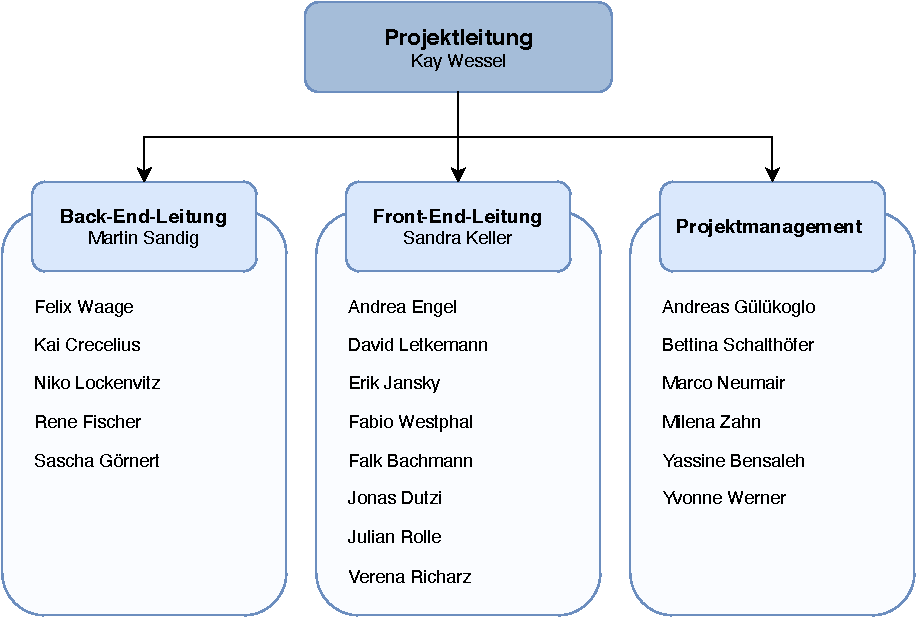
\includegraphics[width=12cm]{img/Organigramm.pdf}
	\captionsetup{format=hang}
	\caption[Organigramm des Projektteams]{\label{fig:Organigramm}Organigramm des Projektteams}
\end{figure}

Zusätzlich zu dem Projektteam gibt es weitere Stakeholder, die an dem Projekt beteiligt sind.
Dazu zählen Herr Prof. Dr. Matt, Herr Prof. Dr. Ritterbusch und Herr Prof. Dr. Reichwald, welche die Kunden sowie Nutzer der Anwendung sind.
Die Betreuung und Bewertung des Projekts erfolgt durch Herrn Becker.



 


\section{Zeitplanung}\label{ch:zeitplanung}
Für die Planung und Kontrolle des Projektfortschritts wurde pro Semester ein Zeitplan erstellt.
Die folgenden Gantt-Diagramme des 5. und 6. Semesters geben einen groben Überblick über diese.
Für das 5. Semester (siehe Abbildung \vref{fig:Gantt5}) wurden verschiedene Zeiträume aufgestellt, jedoch ohne inhaltliche Ziele.
Dem Zeitplan des 6. Semesters (siehe Abbildung \vref{fig:Gantt6}) wurden für die jeweiligen Zeitabschnitte inhaltliche Ziele hinzugefügt, wodurch der Fortschritt des Projekts besser kontrolliert werden konnte.

\begin{figure}[H]
	\centering 
	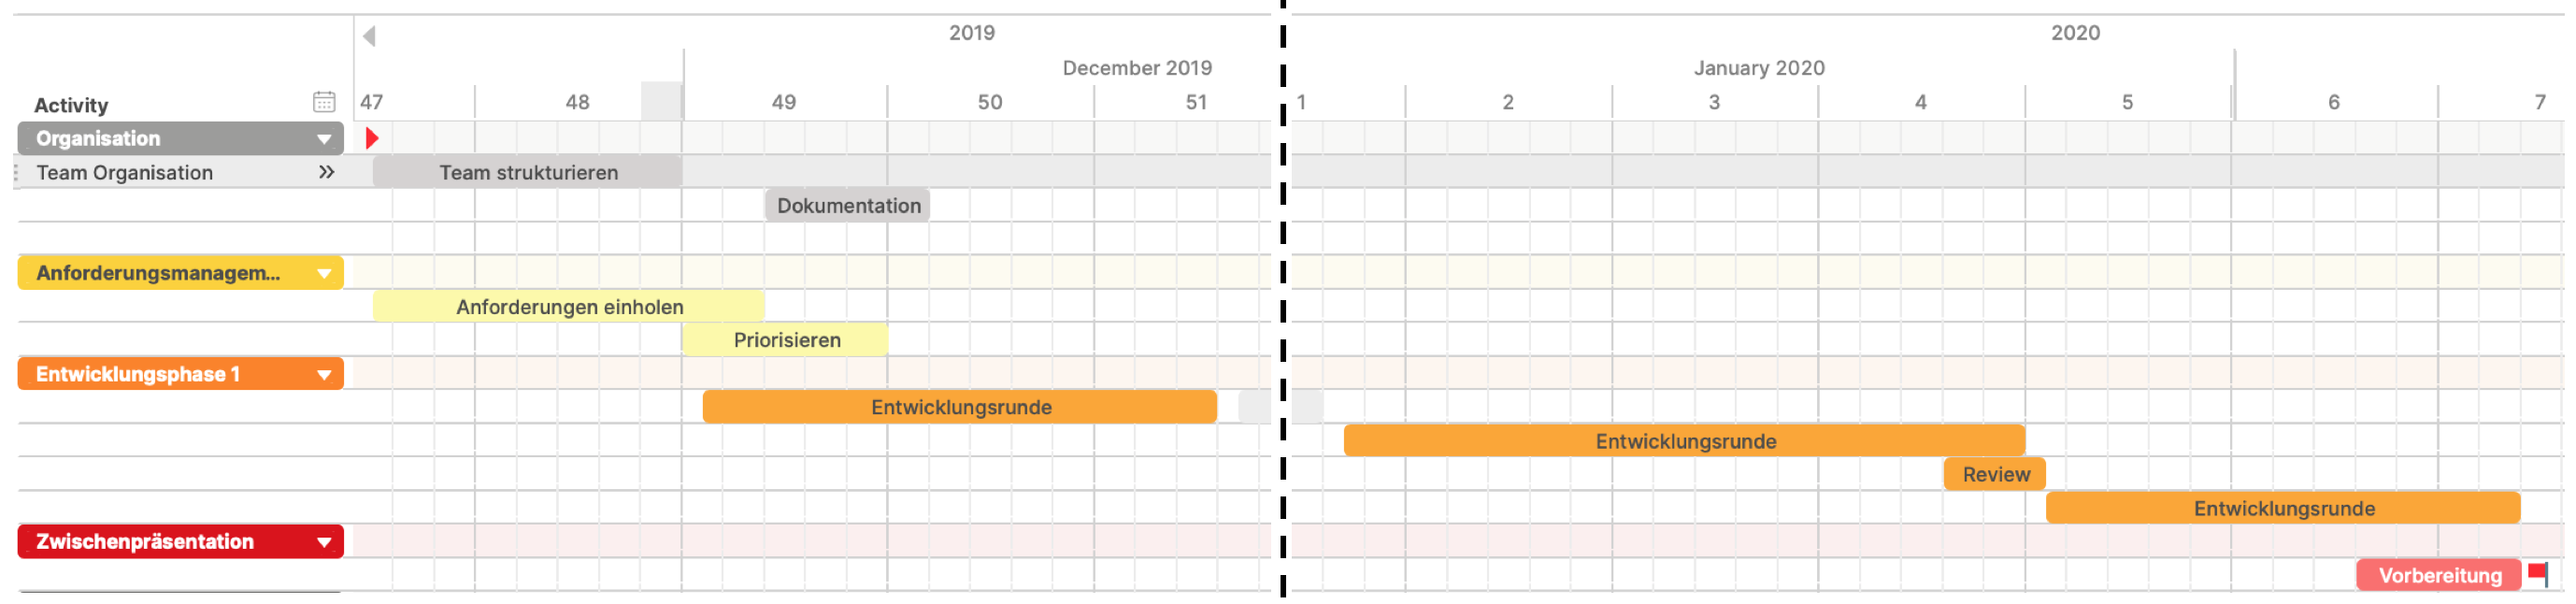
\includegraphics[width=\textwidth]{img/GanttSemester5.png}
	\captionsetup{format=hang}
	\caption[Grobe Übersicht Gantt-Diagramm Semester 5]{\label{fig:Gantt5}Grobe Übersicht Gantt-Diagramm Semester 5}
\end{figure}

\begin{figure}[H]
	\centering 
	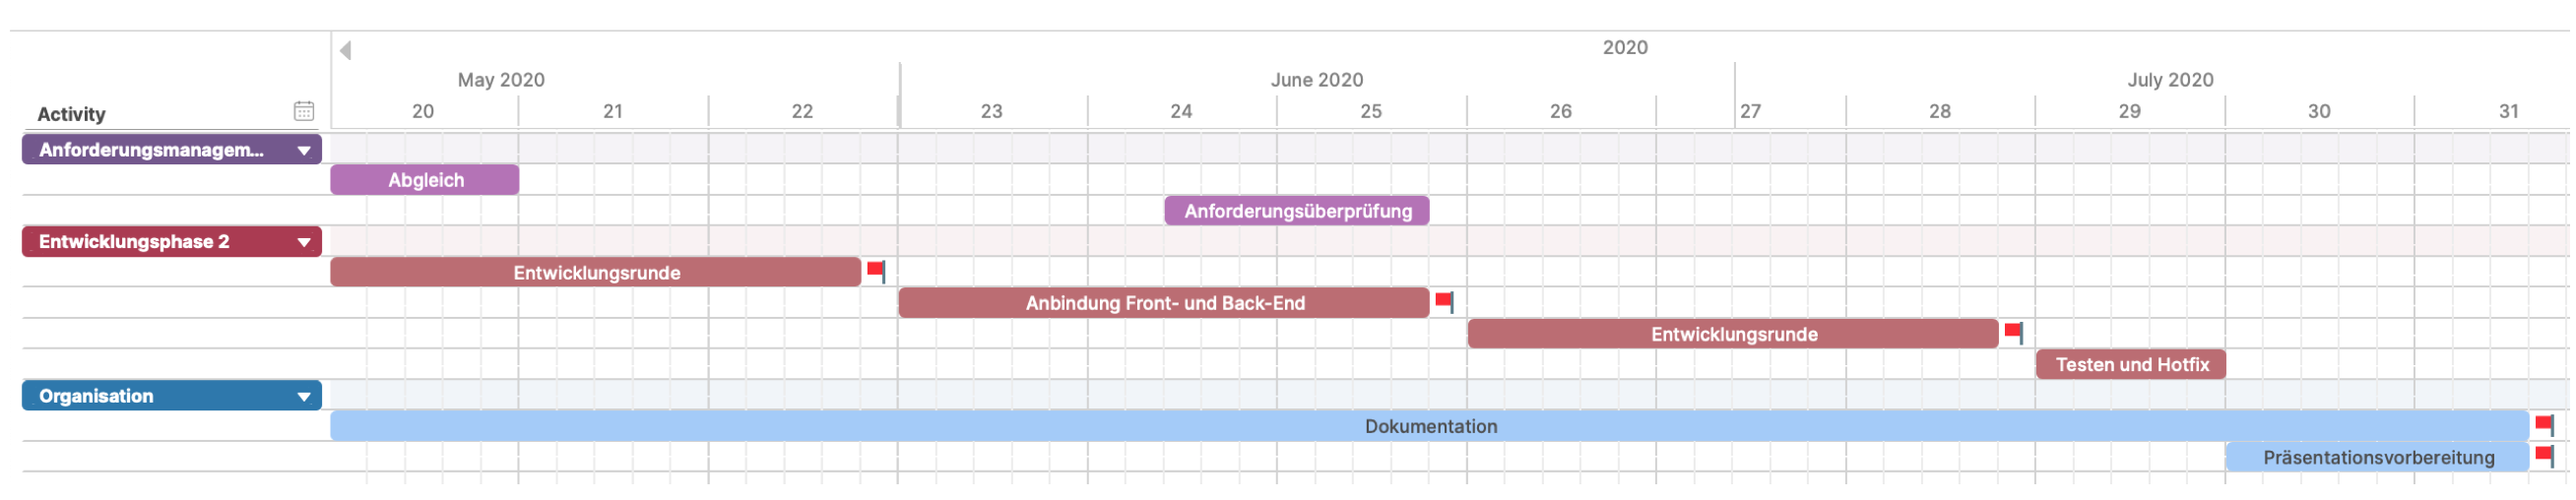
\includegraphics[width=\textwidth]{img/GanttSemester6.png}
	\captionsetup{format=hang}
	\caption[Grobe Übersicht Gantt-Diagramm Semester 6]{\label{fig:Gantt6}Grobe Übersicht Gantt-Diagramm Semester 6}
\end{figure}


\section{Teamorganisation}
%TODO check Projektbeteiligte (Redundanzen)
Zunächst wurde als Projektleiter Kay Wessel festgelegt, der die gesamte Verantwortung für das Projekt trägt und deshalb die oberste Entscheidungsgewalt inne hat. 
Zu seinen Aufgaben gehört die Gesamtplanung des Projekts und das Managen von organisatorischen Angelegenheiten, wie Aufsetzen und Durchführung von Meetings sowie das Klären von inhaltlichen Fragen.

Für das Projekt konnten die drei Aufgabenbereichen Produktmanagement, Front-End und Back-End identifiziert werden.
Anhand dieser Aufgabenbereiche wurde der Kurs in drei dedizierte Teams unterteilt, welche jeweils der Führung eines Teamleiters unterliegen.
Für das Produktmanagement ist Kay Wessel zuständig, Sandra Keller für das Front-End und Martin Sandig für das Back-End.
Die Aufgabe der Teamleiter ist die Verteilung und Kontrolle von Aufgaben unter den jeweiligen Mitgliedern eines Teams.
Das Planen und Erfassen der Aufwände fällt ebenfalls in ihren Tätigkeitsbereich.

Die Organisation und Realisierung des Projektes erfolgte mittels der Nutzung unterschiedlicher digitaler Medien.
Als Unterstützung agiler Softwareentwicklung wurden GitHub sowie Trello verwendet. 
Der netzbasierter Dienst \textit{GitHub}\footnote{\url{https://github.com/}} ermöglicht gemeinsames Arbeiten und die Versionsverwaltung bei Software-Entwicklungsprojekten. 
Für die Entwicklung des Front-End und Back-End sowie für die Erstellung der Dokumentation werden eigene Verzeichnisse (Repositories) verwendet. 

Der Aufgaben-Verwaltungs-Onlinedienst \textit{Trello}\footnote{\url{https://trello.com/}} ermöglicht das Verwalten von Aufgaben in sogenannten Boards. 
Die Aufgaben können beliebig bearbeitet und mit Checklisten, Anhängen, Terminen und vielem mehr versehen werden.
Außerdem lassen sich die Bearbeiter zu einer Aufgabe hinzufügen, sodass diese über alle Änderungen und Fortschritte informiert werden.
Für jedes Team wurde in Trello ein eigenständiges Board erstellt, sodass die Aufgaben im Verbund eines Teams entsprechend zugeordnet und anschließend bearbeitet werden können. 
Zur Klärung allgemeiner Fragen wurde ein gemeinsames Board \enquote{Organisation} eingerichtet.
Da für das Projekt eine Protokollierung der Stunden erforderlich ist, wurde ein geteiltes \textit{Google-Sheet}\footnote{\url{https://www.google.com/sheets/about/}} erstellt, welches das aktuelle Stundenkontingent der Teammitglieder beinhaltet. 
Dieses und die Aufgabenverwaltung mit Trello gewährleisten die Transparenz über die aktuellen Aufwände und Aufgaben. 

Die Kommunikation und Koordination erfolgte über den Instant-Messaging-Dienst \textit{WhatsApp}\footnote{\url{https://www.whatsapp.com/}} sowie das Konferenzsystem \textit{Discord}\footnote{\url{https://discord.com/}}.
In Letzterem sind verschiedene Sprachkanäle eingerichtet, in denen telefonische Absprachen durchgeführt werden können.
Dabei besteht die Möglichkeit den Bildschirm und damit Inhalte zu teilen, welches unter anderem für das gemeinsame Bearbeiten von Aufgaben genutzt wurde. 


\section{Interne Aufgabenverteilung}
- regelmäßigen Meetings
- Springer für FE und BE 

%\section{Projektabschluss}


\chapter{Anforderungsanalyse}
\label{ch:Anforderungsanalyse}
In diesem Kapitel wird die Anforderungsanalyse erstellt.
Zunächst wird die zu lösende Problemstellung sowie die Zielsetzung des Projekts beschrieben.
Anschließend werden die Anforderungen des Auftraggebers identifiziert.
Alle Anforderungen werden danach anhand ihrer Relevanz und dem gegebenen zeitlichen Budget priorisiert.


\section{Ist-Analyse und Zielsetzung}\label{sec:probl}

Die Vorlesungspläne für die Kurse des Studiengangs Wirtschaftsinformatik an der \ac{DHBW} müssen aktuell vollständig manuell durch die jeweiligen Tutoren erstellt werden.
Eine Excel-Vorlage dient dabei als Unterstützung, indem darin Informationen über den Kurs und die Module gesammelt werden.
Für die zu haltenden Vorlesungen müssen passende Dozenten gesucht und angefragt werden, wobei keine zentrale Liste der Dozenten existiert, was den Prozess wiederum erschwert.
Wurden zu allen Vorlesungen passende Dozenten sowie Zeitfenster gefunden, werden diese in einem Google Calendar integriert.

Mit Hilfe eines Tools soll künftig das eben beschriebene Vorgehen zur Erstellung der Vorlesungspläne mit seinen manuellen Teilprozessen für die Studiengangsleiter erleichtert werden.
Ziel dabei ist es, eine zentrale Dozentenverwaltung zu realisieren sowie den Studiengangsleitern ein einheitliches System zur Planung und Koordination ihrer Kurse zur Verfügung zu stellen.


\section{Anforderungen}

Bevor der Lösungsansatz für die Problemstellung aus Kapitel \vref{sec:probl} konzipiert wird, müssen die Wünsche und Vorstellungen des Auftraggebers ermittelt werden.
Bei dem Auftraggeber handelt es sich um einen Studiengangsleiter des Studiengangs Wirtschaftsinformatik an der \ac{DHBW}.
Durch verschiedene Interviews wurden die Anforderungen des Auftraggebers festgestellt.
Die Anforderungen sind in der nachfolgenden Tabelle, Tabelle \ref{tab:Anforderungen}, aufgelistet.

\begin{longtable}[h]{|p{2,5cm}|p{4cm}|p{6,5cm}|}		
	\multicolumn{3}{|r|}{\textit{Fortsetzung nächste Seite}} \\ \hline
	\endfoot
	\endlastfoot
	\hline &&\\[-0.5em]
	\textbf{Anforderung} & \head{Kurztitel} & \head{Beschreibung} \\ \hline
	\endfirsthead
	\hline &&\\[-0.5em]
	\textbf{Anforderung} & \head{Kurztitel} & \head{Beschreibung} \\ \hline
	\endhead
	\parbox[t]{3cm}{A1} & Dozentenpool & Alle Dozenten sollen in einem zentralen Dozentenpool verwaltet werden können.\label{anf:Dozenten}\\ \hline
	\parbox[t]{3cm}{A2} & Stundenplan & Die Software soll Stundenpläne verwalten und erzeugen anhand diverser Parameter, die eingetragen werden wie z.\,B. welche Vorlesungen in welchem Semester für einen Kurs und Dozenten stattfinden.\\ \hline
	\parbox[t]{3cm}{A3} & Google Calendar & Google Calendar soll vollständig in die Software integriert werden.\label{anf:GC}\\ \hline
	\parbox[t]{3cm}{A4} & Profilzuordnung & Die Profile der User, mit denen sie sich am System anmelden, sollen über deren  Mail-Adresse zugeordnet werden.\label{anf:Profilzuordnung}\\ \hline
	\parbox[t]{3cm}{A5} & Modulkataloge & Die Modulkataloge mit den Vorlesungen, Stundenanzahlen und Prüfungsmöglichkeiten (Klausur, Referat oder andere Ausarbeitungen) sollen verwaltet und über Templates hinzugefügt werden können.\label{anf:Modulkatalog} \\ \hline
	\parbox[t]{3cm}{A6} & Kurskoordination & Ein Studiengangsleiter soll eine variable Anzahl an Kursen im System koordinieren können.\\ \hline
	\parbox[t]{3cm}{A7} & Eindeutigkeit der Module & Module müssen eindeutig identifizierbar sein, da z.\,B. das Statistikmodul für Wirtschaftsinformatiker nicht gleich dem Statistikmodul für angewandte Informatiker ist.\\ \hline
	\parbox[t]{3cm}{A8} & Suchen und Filtern im Dozentenpool & In dem Dozentenpool sollen Dozenten per Suche gefunden sowie nach sinnvollen Kriterien gefiltert werden können.\\ \hline
	\parbox[t]{3cm}{A9} & Hinzufügen und Löschen im Dozentenpool & In dem Dozentenpool sollen neue Dozenten hinzugefügt und bestehende Dozenten gelöscht werden können.\\ \hline
	\parbox[t]{3cm}{A10} & Dozenteninformationen im Dozentenpool & Zu jedem Dozenten im Dozentenpool sollen Informationen wie Name, Mail, Handynummer verfügbar sein. Zudem sollen Felder für eine Bewertung, eine Information, ob der Dozent hauptamtlich tätig ist und der/die jeweilige(n) Schwerpunkt(e) sowie ein Freitextfeld für Kommentare vorhanden sein.\\ \hline
	\parbox[t]{3cm}{A11} & Automatisierte Dozentenanfrage & Nach Auswahl eines Dozenten soll diesem automatische eine Anfrage via Mail geschickt werden, wobei ein personalisierbares Template als Basis dient.\\ \hline
	\parbox[t]{3cm}{A12} & Zuordnung der Dozenten & Die Dozenten sollen jeweils einem Studiengangsleiter zugeordnet werden.\\ \hline
	\parbox[t]{3cm}{A13} & Warnung bei maximaler Stundenanzahl & Das Tool soll benachrichtigen, wenn ein Dozent seine maximale Stundenanzahl überschreiten würde bei der aktuellen Planung.\\ \hline
	\parbox[t]{3cm}{A14} & Paralleler Zugriff & Parallele Zugriffe auf einen Kurs durch jeweils berechtigte Personen sollen möglich sein.\\ \hline
	\parbox[t]{3cm}{A15} & Tooladministration & Die Administration des Tools soll über die Studiengangsleiter erfolgen.\\ \hline
	\parbox[t]{3cm}{A16} & Kursübersicht & Es soll pro Kurs eine Übersicht mit Anzahl und Art der jeweiligen Prüfungsleistungen des Kurses existieren.\\ \hline
	\parbox[t]{3cm}{A17} & Farbiger Planungsstand & Der aktuelle Stand der Semesterplanung eines Kurses soll mithilfe von Farben verdeutlicht werden, z.\,B. grün – Termin der Vorlesung ist fix; gelb – Dozent hat zugesagt, aber noch kein fixer Termin; etc.\\ \hline
	\parbox[t]{3cm}{A18} & Planungsexport & Existierende Planungen sollen exportiert werden können, z.\,B. für nachfolgende Kurse.\\ \hline
	\parbox[t]{3cm}{A19} & Informationen der Veranstaltungen & Die detaillierten Informationen über die Veranstaltungen eines geplantes Kurses sollen mithilfe von angehängten Dokumenten einsehbar sein.\\ \hline
	\parbox[t]{3cm}{A20} & Veranstaltungstitel & Der Titel einer Veranstaltung soll in folgender Form dargestellt werden: \enquote{Name der Veranstaltung - Name des Dozenten}.\\ \hline
	\parbox[t]{3cm}{A21} & Automatisierte Benachrichtigungen & Kurse und Dozenten werden mit einer automatisch generierten E-Mail über Semesterbeginn, die finalisierte Planung  oder die Festlegung von Prüfungsterminen und -arten benachrichtigt.\\ \hline
	\parbox[t]{3cm}{A22} & Klausurenmaximum & Das Tool soll berücksichtigen, dass Studiengänge ab 2018  nur sechs schriftliche Klausuren pro Semester erlauben, indem eine entsprechende Warnung ausgegeben wird bei einer Überschreitung.\\ \hline
	\parbox[t]{3cm}{A23} & Korrekte Moduldurchführung  & Die Anwendung soll berücksichtigen, dass Lehrveranstaltungen eines Moduls innerhalb eines Studienjahres erfolgen müssen. Innerhalb eines Studienjahres sollen die Lehrveranstaltungen beliebig verschoben werden können.\\ \hline
	\parbox[t]{3cm}{A24} & Eintragung von Wahlmodulen & Wahlmodule sollen in den Modulkatalog eingetragen werden können.\\ \hline
	\parbox[t]{3cm}{A25} & Dozentenvorschläge & Bei neu hinzugefügten Modulen sollen Vorschläge für den Dozenten generiert werden.\\ \hline
	\parbox[t]{3cm}{A26} & Weiterführbarkeit & Die Software soll später von nachkommenden Jahrgängen weitergeführt und modifiziert werden können.\\ \hline
	\parbox[t]{3cm}{A27} & Usability & Die Bedienbarkeit der Software soll so intuitiv und einfach wie möglich gestaltet werden.\\ \hline
	
	\captionsetup{format=hang}
	\caption[Anforderungen des Auftraggebers]{\label{tab:Anforderungen}Anforderungen des Auftraggebers\\Quelle: Interview mit Professor Matt}
\end{longtable}


\section{Priorisierung}
Die Anforderungen werden, um sie zu priorisieren, in zwei Kategorien eingeteilt.
Als \textit{Muss} wird eine Anforderung kategorisiert, wenn sie die höchste Priorität hat.
Eine Nicht-Erfüllung einer Anforderung, die mit einem \textit{Muss}-Kriterium versehen wurde, kann die Ablehnung des gesamten Projektes oder Produktes bedeuten.
Die \textit{Kann}-Anforderungen sind Abstufungen der \textit{Muss}-Anforderungen und \enquote{können} erfüllt werden, soweit die Ressourcen dies ermöglichen.
Die Anforderungen mit ihren jeweiligen Priorisierungen sind in Tabelle \vref{tab:prios} dargestellt. 

\begin{table}[h]
	\centering
	\renewcommand*{\arraystretch}{1.25}
	\begin{tabular}{|l|p{8cm}|l|}
		\hline &&\\[-0.5em]
		\textbf{Anforderung} & \head{Kurztitel} & \textbf{Priorität} \\ \hline
		A1 & Dozentenpool & \textit{Muss} \\ \hline
		A2 & Stundenplan & \textit{Muss} \\ \hline
		A3 & Google Calendar & \textit{Muss} \\ \hline
		A4 & Profilzuordnung & \textit{Muss} \\ \hline
		A5 & Modulkataloge & \textit{Muss} \\ \hline
		A6 & Kurskoordination & \textit{Muss} \\ \hline
		A7 & Eindeutigkeit der Module & \textit{Muss} \\ \hline
		A8 & Suchen und Filtern im Dozentenpool & \textit{Muss} \\ \hline
		A9 & Hinzufügen und Löschen im Dozentenpool & \textit{Muss} \\ \hline
		A10 & Dozenteninformationen im Dozentenpool & \textit{Muss} \\ \hline
		A11 & Automatisierte Dozentenanfrage & \textit{Kann} \\ \hline
		A12 & Zuordnung der Dozenten & \textit{Kann} \\ \hline
		A13 & Warnung bei maximaler Stundenanzahl & \textit{Kann} \\ \hline
		A14 & Paralleler Zugriff & \textit{Kann} \\ \hline
		A15 & Tooladministration & \textit{Kann} \\ \hline
		A16 & Kursübersicht & \textit{Kann} \\ \hline
		A17 & Farbiger Planungsstand & \textit{Kann} \\ \hline
		A18 & Planungsexport & \textit{Kann} \\ \hline
		A19 & Informationen der Veranstaltungen & \textit{Kann} \\ \hline
		A20 & Veranstaltungstitel & \textit{Kann} \\ \hline
		A21 & Automatisierte Benachrichtigungen & \textit{Kann} \\ \hline
		A22 & Klausurenmaximum & \textit{Kann} \\ \hline
		A23 & Korrekte Moduldurchführung & \textit{Kann} \\ \hline
		A24 & Eintragung von Wahlmodulen & \textit{Muss} \\ \hline
		A25 & Dozentenvorschläge & \textit{Kann} \\ \hline
		A26 & Weiterführbarkeit & \textit{Kann} \\ \hline
		A27 & Usability & \textit{Muss} \\ \hline
	\end{tabular}
	\captionsetup{format=hang}
	\caption{\label{tab:prios}Priorisierung der Anforderungen \\}
\end{table}








\chapter{Entwurf}\label{ch:Entwurf}


\section{Design Entwurf}\label{ch:DesignEntwurf}

Für das Design sollte ein Prototyp erstellt werden, der den späteren Aufbau der Applikation verdeutlicht.
Als technisches Hilfsmittel wurde das cloud-basierte Tool \textit{Figma}\footnote{\url{https://www.figma.com/}} verwendet.
Dieses bietet die Möglichkeit mit mehreren Personen in Echtzeit an einem Prototypen zu arbeiten.
Dabei ist es in seiner Bedienung leicht verständlich und bietet alle wichtigen Design-Werkzeuge. 
Außerdem können die Elemente der Benutzeroberfläche miteinander verbunden und mit Interaktionen sowie Animationen versehen werden, sodass ein interaktiver Prototyp entsteht.
Nach dem Starten eines Prototyps kann das Design der Oberfläche sowie die Navigationen geprüft werden.
Über einen generierten Link lässt sich der Prototyp mit Projektbeteiligten teilen. 

Für das Erstellen des Designs wurde eine iterative Vorgehensweise gewählt.  
Gestartet ist der Prozess mit dem Einholen von Anforderungen, siehe Kapitel \ref{ch:Anforderungsanalyse}.
Basierend darauf konnte die allgemeine Struktur der Benutzeroberfläche erstellt werden.
Anschließend verlief der Prozess in vielen Iterationsschleifen, in denen bekannte Anforderungen zunächst statisch umgesetzt und bei Rücksprachen mit den Stakeholdern deren Feedback eingeholt wurde.
Dabei wurden ebenfalls weitere Anforderungen besprochen, sodass das Design nachfolgend erweitert werden konnte.
Während den Schleifen wurde der Prototyp jeweils interaktiv erstellt, d.h. mit Animationen versehen, und es wurden weitere Details hinzugefügt.
Auf diese Weise sind während dem Projekt verschiedene Versionen des Prototyps entstanden, die jeweils mit den Stakeholdern besprochen wurden.
Neben diesen Absprachen erfolgten zusätzliche mit dem Back-End-Team.
Thema dieser Besprechungen waren die Umsetzbarkeit der Funktionalitäten, die vom Back-End bereitgestellt werden müssen.
Damit aber auch das gesamte Projektteam über den Entwurf und die Fortschritte informiert blieb, wurden das jeweils aktuelle Design in verschiedenen wöchentlichen Meetings des gesamten Teams präsentiert.
Damit jedes Team-Mitglied jederzeit auf den Prototyp zugreifen kann, wurde der Link in Trello eingetragen. 

Die designte Benutzeroberfläche besteht, wie in Abbildung \ref{fig:Seitenaufbau} dargestellt, jeweils aus drei Elementen.
Sie beinhaltet eine Kopfzeile, eine Navigationsleiste und die gewählten Inhalte.
\begin{figure}[h]
	\centering 
	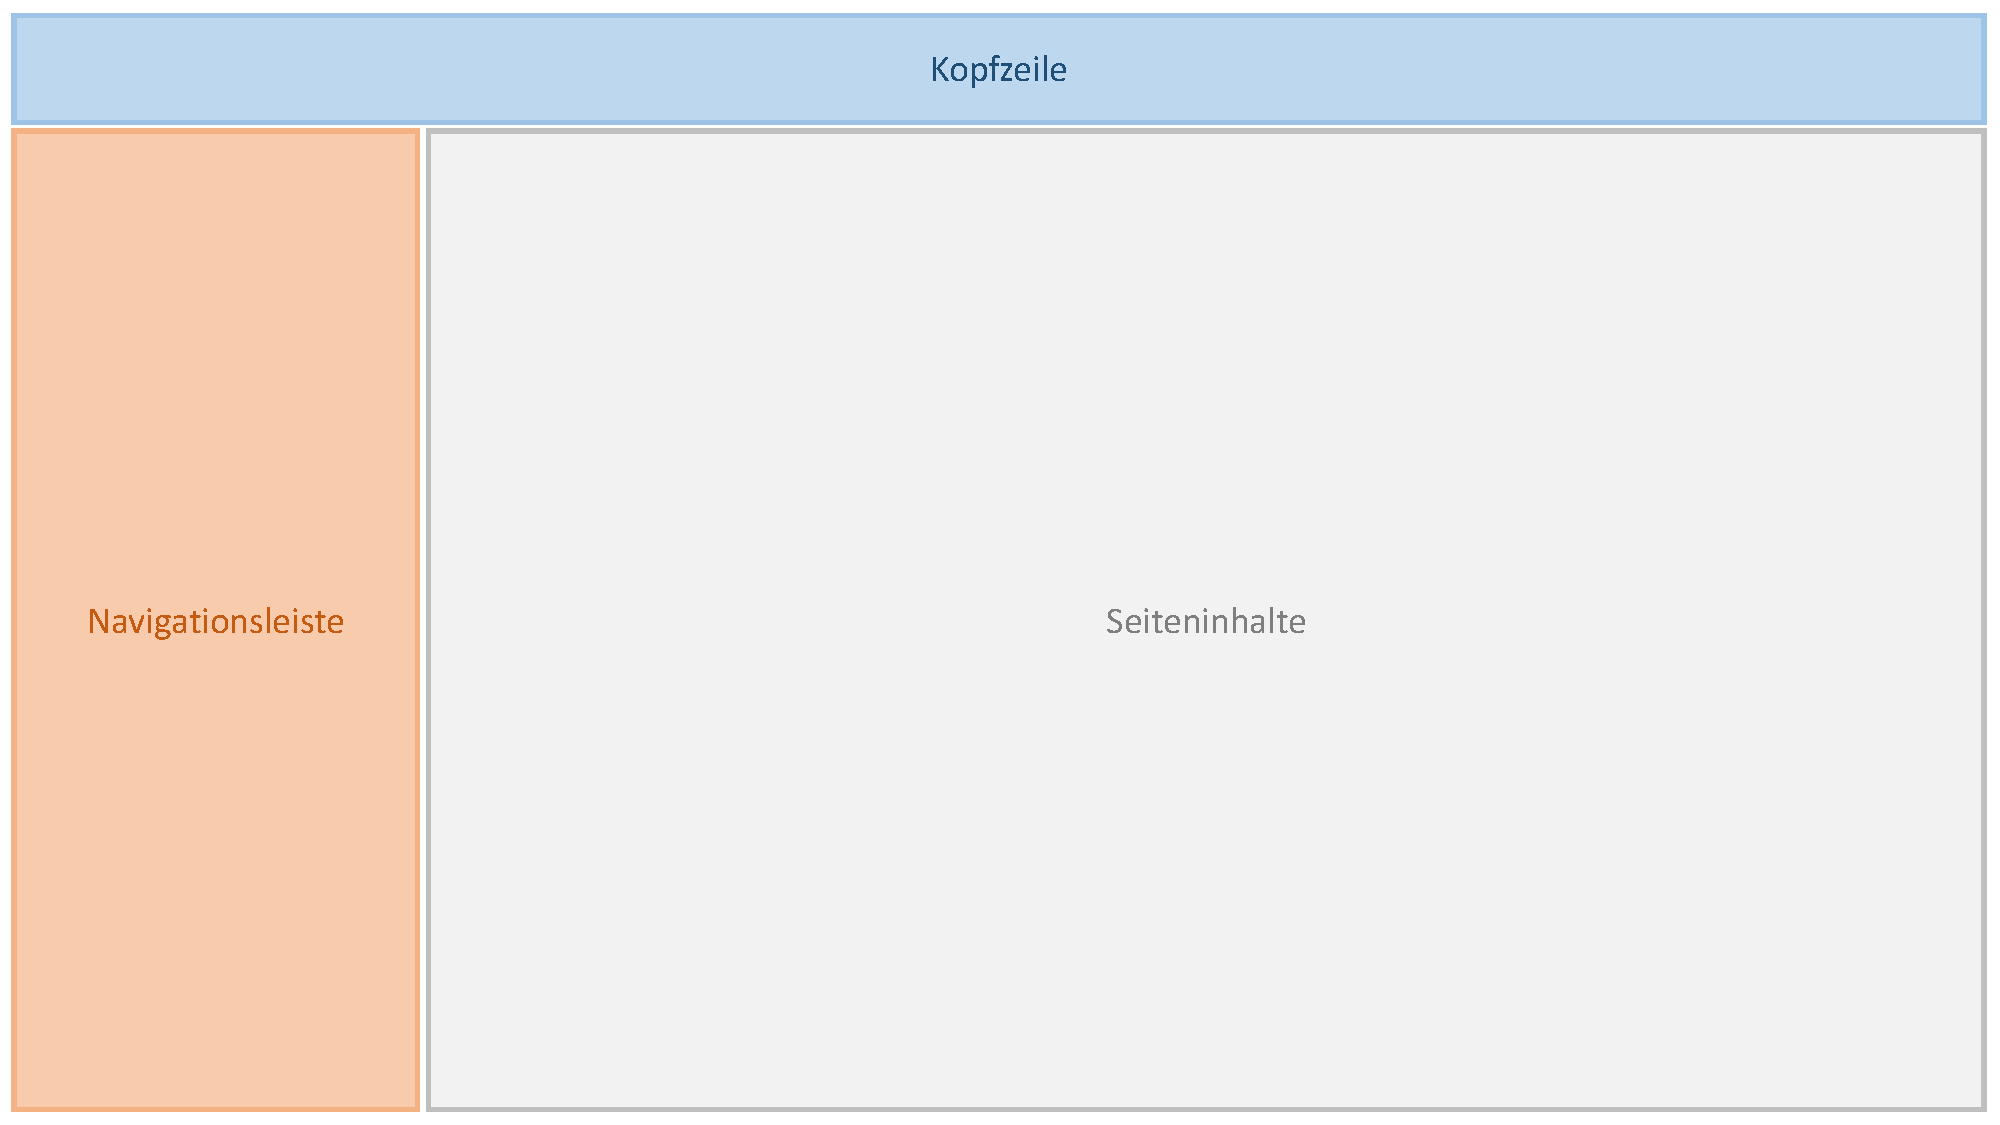
\includegraphics[width=\textwidth]{img/Seitenaufbau.pdf}
	\captionsetup{format=hang}
	\caption[Aufbau der Benutzeroberfläche]{\label{fig:Seitenaufbau}Aufbau der Benutzeroberfläche}
\end{figure}
Die Kopfzeile stellt am linken Rand das Logo der \acs{DHBW} und am rechten Rand den Benutzernamen dar.
Durch das Anklicken des Benutzernamens können allgemeine Kontoeinstellungen getätigt oder das Abmelden von der Applikation ausgelöst werden.
Auf jeder Seite der Benutzeroberfläche befindet sich außerdem am linken Rand eine vertikale Navigationsleiste.
Diese beinhaltet die vier Hauptseiten und ermöglicht das Navigieren zwischen diesen.
Es können die Vorlesungen und Vorlesungspläne je Kurs, eine Übersicht der Dozenten und verschiedene Modulkataloge angeschaut werden. Die Datenverwaltung ermöglicht das Hinzufügen, Ändern und Löschen von Studiengängen, Schwerpunkten und Prüfungsleistungen.

In Abbildung \ref{fig:Mockup} wird eine Hauptseite des Prototyps dargestellt. Das gesamte Mockup ist unter dem \underline{\hyperlink{https://www.figma.com/proto/WZp01tmSA4nxDskhnfqv3x/Fourth-Prototype?node-id=1\%3A2\&scaling=contain}{Link}} zu finden.

\begin{figure}[H]
	\centering 
	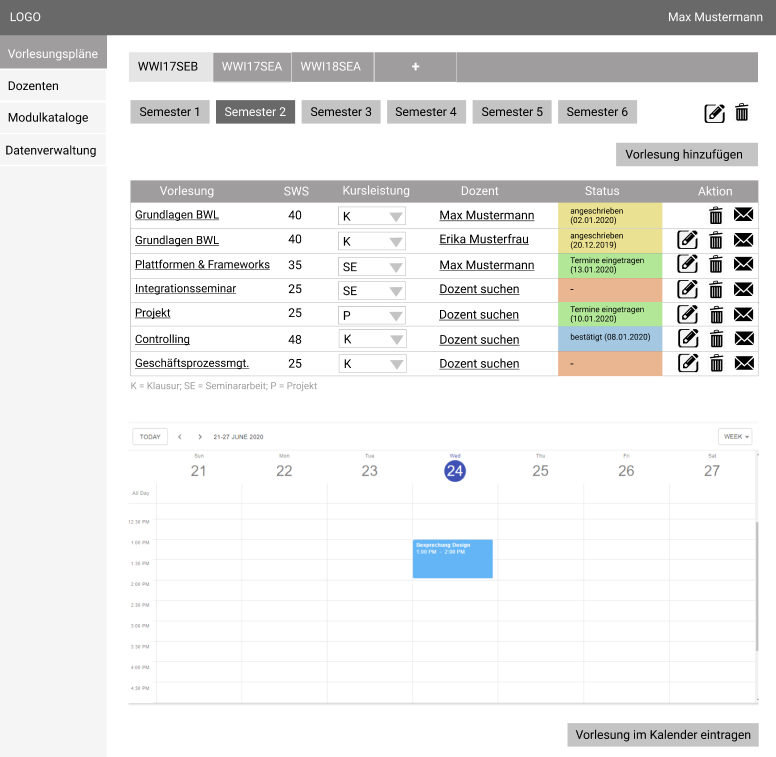
\includegraphics[width=\textwidth]{img/Mockup.PNG}
	\captionsetup{format=hang}
	\caption[Hauptseite ds Prototyps]{\label{fig:Mockup}Hauptseite des Prototyps\footnotemark}
\end{figure}
\footnotetext{\url{https://www.figma.com/proto/WZp01tmSA4nxDskhnfqv3x/Fourth-Prototype?node-id=1\%3A2\&scaling=contain}}


\section{Technischer Entwurf}
\label{ch:Technischer Entwurf}
\subsection{Grundlegende Architektur}
\label{ch:grundlegendeArchitektur}
In Abbildung \vref{fig:Aufbau} ist der grundlengede Aufbau der Webanwendung skizziert.
Dieser besteht aus mehreren Komponenten, die gemäß eines Microservice-Ansatzes unabhängig voneinander bestehen. 
Dies bietet außerdem die Vorteile, dass durch die verringerte Kopplung eine bessere Wartbarkeit der einzelnen Bestandteile gegeben ist sowie diese einfach ersetzt werden können. 
Mithilfe eines Docker-Netzwerks kann dieser Ansatz umgesetzt werden und bietet zusätzlich ein einfaches Deployment der Anwendung. 

\begin{figure}[H]
	\centering 
	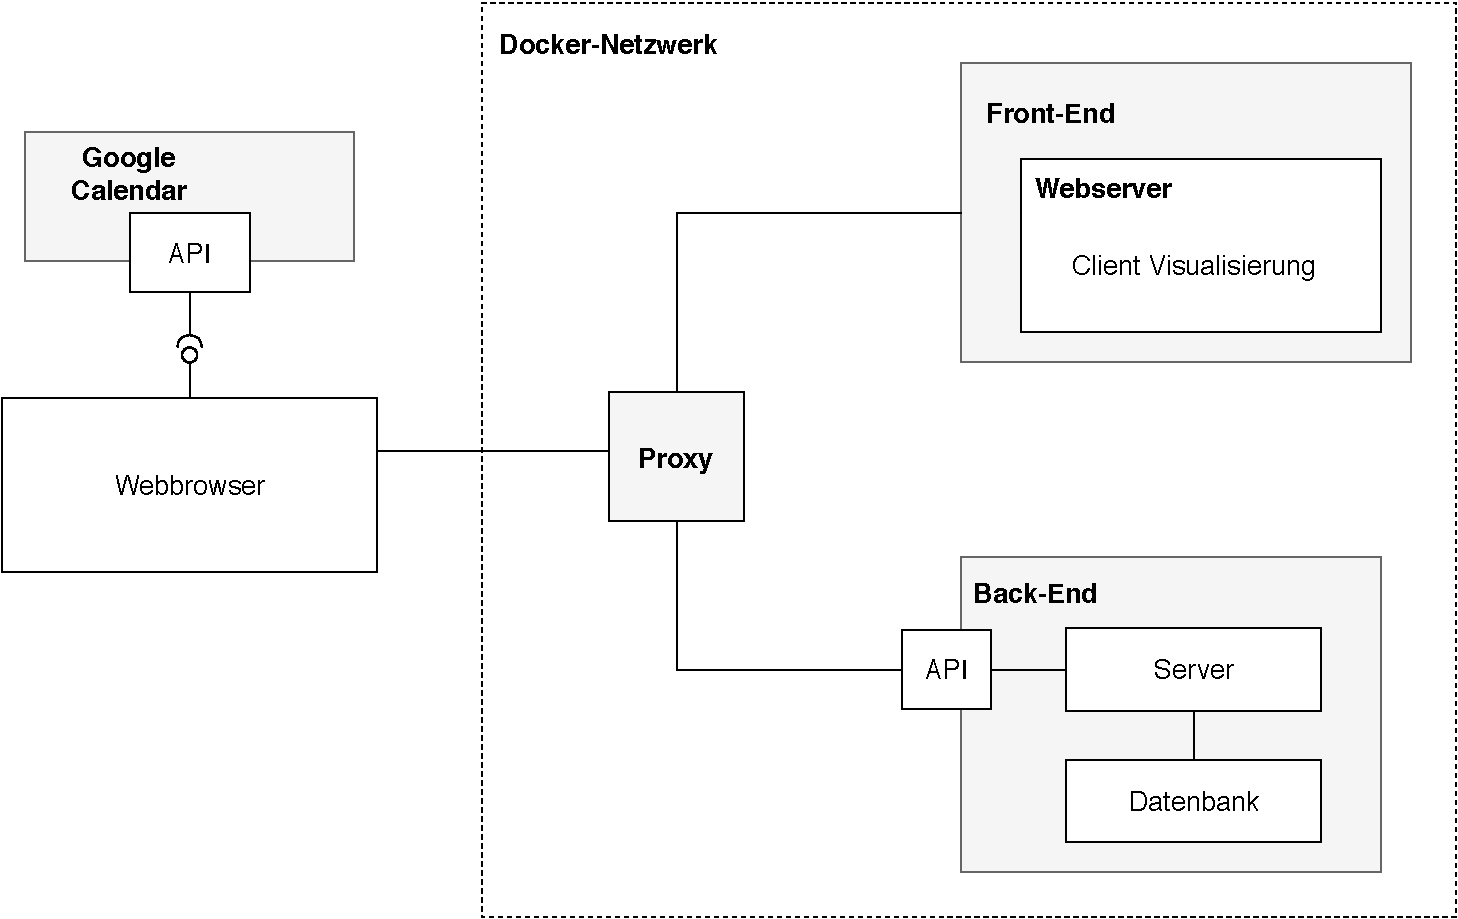
\includegraphics[width=13cm]{img/TechnischerEntwurf.pdf}
	\caption[Grundlegende Architektur]{\label{fig:Aufbau}Grundlegende Architektur}
\end{figure}

Die Abbildung stellt eine Übersicht über den Aufbau dar und bietet eine logische Trennung der Komponenten. 
Allgemein lassen sich folgende Hauptkomponenten unterscheiden:
\begin{itemize}
    \item Front-End zur Bereitstellung der Benutzeroberfläche an den Webbrowser des Clients 
    \item Back-End zur Datenhaltung und Geschäftslogik
    \item Proxy als Kommunikationsschnittstelle
    \item Webbrowser mit einer Anbindung an die Google Calendar-Schnittstelle.
\end{itemize} 

Das Front- und Back-End sollen als eigenständige Microservices mit eigenem Server umgesetzt werden, sodass die Entwicklung der Komponenten losgelöst ablaufen kann und durch andere Technologien ersetzt werden könnte.
Das Front-End dient zur Bereitstellung der grafischen Benutzeroberfläche und wird an den Webbrowser des Clients ausgeliefert. 
Das Back-End hingegen besteht aus einem Server mit der Geschäftslogik sowie einer Datenbank zur Datenhaltung der Anwendung. 
Diese Dienste sollen über eine \ac{API} erreichbar sein. 
Der Proxy stellt die zentrale Schnittstelle der Webanwendung dar und liefert das Front-End aus. 
Von dem Webbrowser wird außerdem auf die externe Schnittstelle des Google Calendars zugegriffen, um eine Verbindung zu einem Google Calendar gemäß der Anforderung A2 und A3 aus der Tabelle \ref{anf:GC} herzustellen.


\subsection{Datenmodell}
Für das serverseitige Speichern von Daten sind relationale Datenbanken weit verbreitet.
Deshalb wird auch im Rahmen dieses Projekts eine solche Form der Datenhaltung genutzt.
Im Folgenden wird nun das Datenmodell näher erläutert, welches im Anhang \vref{fig:ermodell} dargestellt ist.  

Über \texttt{directorOfStudies} werden die Nutzer der Anwendung, die Studiengangsleiter, dargestellt.
Sie sind nicht automatisch als Dozenten hinterlegt, können jedoch als solche hinzugefügt werden.
Ein Studiengangsleiter kann zusätzlich ein Administrator der Anwendung sein, wodurch er weitere Berechtigungen erhält, wie das Zurücksetzen von Passwörtern.

Die Entität \texttt{course} repräsentiert einen Kurs der \ac{DHBW}, welcher genau einem Studiengang (\texttt{fieldOfStudy}) und einer Studienrichtung (\texttt{majorSubject}) zugeordnet ist.
Damit die Eindeutigkeit der Module (Anforderung  A7 aus der Tabelle \ref{anf:GC}) gewährleistet ist, referenziert \texttt{majorSubject} auf die dazugehörigen Modulgruppen und entspricht dadurch dem gegebenen Aufbau des Modulkatalogs.
Aus diesem Grund beinhaltet es auch das Jahr, ab welchem der Modulkatalog gültig ist. 

Damit auch Wahlmodule abgebildet werden können (Anforderung A24 aus der Tabelle \ref{anf:GC}), sind die Module (\texttt{module}) Teil einer Modulgruppe (\texttt{moduleGroup}).
Besteht die Wahlmöglichkeit zwischen mehreren Modulen, beinhaltet die Modulgruppe alle wählbaren Module.
Andernfalls beinhaltet sie nur das vorgesehene Modul.
Damit neben den Informationen des aktuellen Modulkatalogs der \ac{DHBW} auch die Prüfungsleistung je Modul gespeichert werden kann, wird die Entität \texttt{academicRecord} verwendet.

Kurse beinhalten neben ihrem Namen auch eine Referenz auf den für sie angelegten Google Calendar. 
Mithilfe von \texttt{semester} werden die kursspezifischen Semester festgelegt, welche den zeitlichen Rahmen des Studiums beschreiben.
Die Kurse unterliegen üblicherweise einem Studiengangsleiter, jedoch ist es auch möglich weitere Studiengangsleiter hinzuzufügen, beispielsweise für Übergangszeiten bei Positionswechseln.

Die Dozenten (\texttt{lecturer}) werden durch zahlreiche Attribute beschrieben (Anforderung A10 aus der Tabelle \ref{anf:GC}) sowie ein Lebenslauf kann als PDF gesondert gespeichert werden.
Gemäß Anforderung A1 aus der Tabelle \ref{anf:GC} findet die Verwaltung der Dozenten in einem zentralen Dozentenpool statt.
Dabei ist ihnen jeweils genau ein Studiengangsleiter als Ersteller zugeordnet (Anforderung A12 aus der Tabelle \ref{anf:GC}) und die Bearbeitbarkeit durch andere Studiengangsleiter kann eingeschränkt werden. 
Für die Verknüpfung zwischen Dozenten und Vorlesung wird ein thematischer Schwerpunkt (\texttt{mainFocus}) eingesetzt.
Dadurch wird es ermöglicht passende Dozenten für Vorlesungen vorzuschlagen (Anforderung A25 aus der Tabelle \ref{anf:GC}).

Eine \texttt{lecture} ist eine abstrakte Lehr-/Lerneinheit.
Sie beinhaltet lediglich allgemeine Beschreibungen und ist somit für alle Kurse einer Studienrichtung anwendbar. 
Planungseinheiten für konkrete Veranstaltungen werden über die Entität \texttt{presentations} abgebildet.
Sie referenzieren auf abstrakte Vorlesungen, eine Prüfungsleistung sowie ein Semester und einen Kurs. 
Durch Planungseinheiten können gleiche Veranstaltungen mehrfach erzeugt werden, um mehrere Dozenten gleichzeitig zu kontaktieren und anzufragen.
Der Status einer \texttt{presentation} indiziert den Fortschritt der Planung und die Rückmeldungen der jeweiligen Dozenten.





\chapter{Umsetzung}

\section{Infrastruktur}
\subsection{VM}
\subsection{Docker}

\section{Backend}
\subsection{Grundlegender Aufbau}
\label{ch:GrundlegenderAufbau}

\subsubsection{Server}
Zur Implementierung der Geschäftslogik wird ein Webserver mit \textit{Node.js}\footnote{\url{https://nodejs.org/}} und dem Framework \textit{Express}\footnote{\url{https://expressjs.com/}} entwickelt.
Das Framework Express dient der Entwicklung von Webanwendungen und \acp{API}.
Diese Technologien sind weit verbreitet und einigen Teammitgliedern bereits bekannt.
Besonders letzteres spricht für die Nutzung, da keine Einarbeitungsphase notwendig ist und direkt mit der Entwicklung gestartet werden kann. 

\subsubsection{Datenbank}
Das Anbieten der \ac{API}-Endpunkte und den dazugehörigen Funktionen erfordert das serverseitige Speichern von Daten, wie die Studiengangsleiter und Dozenten.
Für die Datenhaltung wurde eine \textit{PostgreSQL}\footnote{\url{https://www.postgresql.org/}} ausgewählt, da sie relational aufgebaut und durch vorige Vorlesungen bereits bekannt ist.
Außerdem ist sie ziemlich verbreitet, weshalb einige Frameworks angeboten werden, die mit Node.js verwendet werden können.
Ein Beispiel dafür ist das \ac{ORM} \textit{Sequelize}\footnote{\url{https://sequelize.org/master/}}, welches in diesem Projekt für die Anbindung der Datenbank an das Back-End verwendet wird.

\subsubsection{Architektur}
Die Architektur des Back-Ends lässt sich durch das in Abbildung \ref{fig:Schichtenmodell} dargestellte Schichtenmodell beschreiben.
Wird eine Anfrage an das Back-End gestellt, erfolgt zunächst die Authentifizierung des Benutzers.
Dazu wird geprüft, ob dieser bereits erstellt wurde und ob der mitgegebene Token dem hinterlegten Token entspricht.
Dadurch kann entschieden werden, ob die mitgegebene Route benutzt werden darf. 

\begin{figure}[h]
	\centering 
	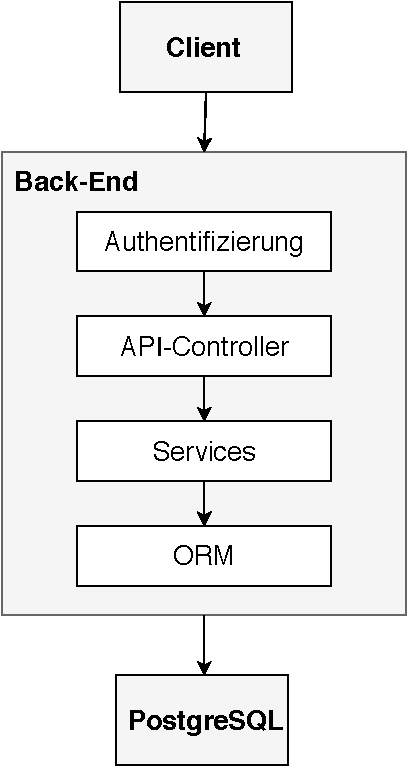
\includegraphics[width=0.4\textwidth]{img/SchichtenmodellBackend.pdf}
	\captionsetup{format=hang}
	\caption[Schichtenmodell des Back-Ends]{\label{fig:Schichtenmodell}Schichtenmodell des Back-Ends}
\end{figure}

Ist dies der Fall, wird die Anfrage an die nächste Schicht weitergegeben.
Durch die API-Controller werden die Routen abgebildet.
Für jede Route gibt es einen eigenen Controller, welcher die jeweiligen \ac{HTTP}-Methoden einer Route anbietet.
Außerdem enthält diese Schicht eine Steuerlogik, welche prüft, ob die gewünschte Aktion von dem Benutzer durchgeführt werden darf. 

Die Serviceschicht stellt eine Abstraktion von dem Inhalt der Datenbank bereit.
Sie definiert außerdem die \ac{ORM}-Aufrufe und stellt dadurch eine Verbindung zum O/R-Mapper bereit. 

Mithilfe des \ac{ORM} werden die objektorientierten Konzepte auf entsprechende rationale Konzepte abgebildet.
Auf diese Weise können Entwickler in der objektorientierten Programmiersprache bleiben, um auf die Datenbank zuzugreifen.
Dieser Zugriff erfolgt im nächsten Schritt, wo die Daten entsprechend der gestellten Anfrage ausgelesen und an den Benutzer zurückgegeben werden. 

\subsection{API-Schnittstellen}
\subsubsection{Implementierung der Routen}
Für die \ac{API}-Endpunkte wird jeweils eine Funktion aufgerufen, welche die übergebenen Daten entgegennimmt, diese prüft und daraufhin auf Datenbank zugreift.
Dieser Vorgang erstreckt sich über die verschiedenen Schichten des Back-Ends und ist in Kap. \ref{ch:GrundlegenderAufbau} detaillierter beschrieben.
Die Routen sind an dem \ac{REST}-Paradigma orientiert, wonach nur die benötigten Informationen zurückgegeben werden.
Bei den Modulgruppen wurde jedoch davon abgewichen, da ein semantischer Zusammenhang zwischen den einzelnen Modulgruppen besteht.
Bei einem GET-Request werden immer alle Modulgruppen der angegebenen Studienrichtung zurückgegeben.
Dies vereinfacht die Programmierung im Front-End, da mit einer Anfrage an das Back-End alle Informationen zum Anzeigen eines bestimmten Modulkatalog zurückgegeben werden.

Durch die Routen wird der Zugriff auf die vorhanden \ac{REST}-Ressourcen gewährleistet, was unter anderem das Erstellen, Lesen, Bearbeiten und Löschen ermöglicht (CRUD-Operationen).
Für den Zugriff auf die Routen wird das \ac{HTTP}-Protokoll verwendet.
Dadurch können entsprechende Statuscodes von \ac{HTTP} verwendet werden, um eine Rückmeldung zum Erfolg oder Misserfolg einer Anfrage zu geben. 
Liegt eine fehlerhafte Anfrage vor, wird eine spezifische Fehlermeldung mit Erklärung in einem 4xx-Code an den Client gesendet.
Der \ac{HTTP}-Code 500 indiziert einen Fehler, welcher möglicherweise im Back-End liegt.


\subsubsection{Übersicht der Routen}
Die Tabellen \ref{tab:routen} und \ref{tab:adminrouten} geben eine Übersicht der zur Verfügung stehenden Routen und die \ac{HTTP}-Methoden, mit welchen auf die Routen zugegriffen werden kann. 
Tabelle \ref{tab:routen} beschreibt die Routen und ihre Aktionen, die von allen Nutzern der Anwendung verwendet werden können.
Dazu zählt beispielsweise das nach Anforderung \hyperref[tab:Anforderungen]{A9} geforderte Anlegen und Löschen von Dozenten, welches mithilfe der Route \texttt{$\backslash$lecturers} durchgeführt wird.

\begin{table}[h]
	\centering
	\renewcommand*{\arraystretch}{1.25}
	\begin{tabular}{|l|P{2cm}|P{2cm}|P{2cm}|P{2cm}|}
		\hline &&\\[-0.6em]
		\textbf{Route} & \textbf{GET} & \textbf{POST} & \textbf{PUT} & \textbf{DELETE} \\ \hline
		$\backslash$register & & x & & \\ \hline
		$\backslash$login & & x & & \\ \hline
		$\backslash$changePassword & & & x & \\ \hline
		$\backslash$academicRecords & x & x & x & x \\ \hline
		$\backslash$courses & x & x & x & x \\ \hline
		$\backslash$directorOfStudies & x & & x & \\ \hline
		$\backslash$fieldsOfStudy & x & x & x & x \\ \hline
		$\backslash$googleCalendarAPI & x & & & \\ \hline
		$\backslash$lecturerCV & x & & x & x \\ \hline
		$\backslash$lecturers & x & x & x & x \\ \hline
		$\backslash$mainFocuses & x & x & x & x \\ \hline
		$\backslash$majorSubjects & x & & x & x \\ \hline
		$\backslash$modulecatalog & x & & & \\ \hline
		$\backslash$moduleGroups & & x & x & x \\ \hline
		$\backslash$presentations & x & x & x & x \\ \hline
		$\backslash$semesters & & x & x & x \\ \hline
		$\backslash$transferOwnership & & x & & \\ \hline
	\end{tabular}
	\captionsetup{format=hang}
	\caption{\label{tab:routen}Übersicht Routen \\}
\end{table}

In Tabelle \ref{tab:adminrouten} werden hingegen die Routen und Aktionen veranschaulicht, welche nur von Administratoren verwendet werden können.
Diese umfassen unter anderem das Anlegen und Auslesen von Nutzern.
Außerdem kann ein Google Calendar aktualisiert und ein Nutzer zu einem Admin ernannt werden. 

\begin{table}[h]
	\centering
	\renewcommand*{\arraystretch}{1.25}
	\begin{tabular}{|l|P{2cm}|P{2cm}|P{2cm}|P{2cm}|}
		\hline &&\\[-0.6em]
		\textbf{Admin-Route} & \textbf{GET} & \textbf{POST} & \textbf{PUT} & \textbf{DELETE} \\ \hline
		$\backslash$createUser & & x & & \\ \hline
		$\backslash$googleCalendarAPI & & & x & \\ \hline
		$\backslash$registerKey & x & & x & \\ \hline
		$\backslash$resetPassword & & & x & \\ \hline
		$\backslash$upgradeToAdmin & & & x & \\ \hline
		$\backslash$users & x & & & \\ \hline
	\end{tabular}
	\captionsetup{format=hang}
	\caption{\label{tab:adminrouten}Übersicht Admin-Routen \\}
\end{table}

Während der Entwicklung wurden weitere Routen erstellt.
Die Entscheidungen im Laufe des Projekts haben jedoch dazu geführt, dass diese nicht mehr notwendig sind und deshalb nicht weiter entwickelt wurden.
Ein Beispiel ist die Route \texttt{$\backslash$signup}.
Diese wird mehr angeboten, da eine selbstständige Registrierung nicht mehr ohne Weiteres möglich sein soll.

\subsection{Sicherheit und Zugriffskontrolle}
Da die Anwendung nur von bestimmten Personen verwendet werden soll, wird die Registrierung eingeschränkt.
Dies erfolgt über einen Registrierungsschlüssel, welcher bei einer Registrierung angegeben werden muss.
Ein solcher Schlüssel ist dem Administrator bekannt und er kann einen neuen Registrierungsschlüssel festlegen.
Der Schlüsselaustausch findet mündlich statt.
Soll der Schlüssel jedoch nicht weitergegeben werden, besteht für den Administrator die Möglichkeit Benutzer des Systems selbst hinzuzufügen. 

Des Weiteren sollen in der Anwendung nur benutzerspezifische Inhalte angezeigt werden und ein Benutzer darf nur die Aktionen durchführen, zu denen er berechtigt ist.
Dafür muss ein Nutzer identifiziert werden können, weshalb eine digitale Identität erstellt wird.
Dies erfolgt durch die Registrierung mit Mail-Adresse und Passwort, entsprechend der Anforderung \hyperref[tab:Anforderungen]{A4}.

Für den Abgleich des gespeicherten Passworts und des eingetragenen Passworts bei der Anmeldung eines Nutzers, muss das Passwort gespeichert werden.
Damit dieses nicht ausgelesen und für unberechtigten Zugang zu der Software genutzt werden kann, wird das Passwort als Hash-Wert gespeichert.
Dieser wird mithilfe der Node.js-Bibliothek \textit{bcrypt}\footnote{\url{https://www.npmjs.com/package/bcrypt}} erstellt.
Bcrypt ist eine kryptographische Hashfunktion speziell für Passwörter. 

Um jedoch eine häufige Verwendung des Passworts zu vermeiden wird ein \textit{JSON Web Token}\footnote{\url{https://jwt.io/}} generiert, welches ein genormtes Access-Token darstellt.
Bei der Registrierung und Anmeldung eines Nutzers wird ein solches Token ausgestellt und bei anschließenden Anfragen an das Back-End mitgegeben.
Dieses prüft daraufhin die Korrektheit des Tokens bevor eine Aktion durchgeführt wird.
Ist der Nutzer gespeichert und das Token hinterlegt, ist dieser berechtigt Anfragen zu senden.
Außerdem wird bei jedem Aufruf in den Controllern geprüft, ob eine Aktion valide ist.
Auf diese Weise wird bspw. verhindert, dass ein Studiengangsleiter die Kurse eines anderen ändern kann. 

Ähnlich wie Passwörter nicht im Klartext gespeichert werden sollten, sollte auch die Kommunikation zwischen Client und Server nicht im Klartext erfolgen.
Deshalb wird das Kommunikationsprotokoll \ac{HTTPS} verwendet.
Dadurch werden die Nachrichten verschlüsselt übertragen, was insbesondere für die Übermittlung von Passwörtern und Token wichtig ist. 
\newpage
\section{Front-End}
\label{ch:FrontEnd}
\subsection{Implementierung mit React}
Zur Erstellung des Front-Ends der Webanwendung wird \textit{React}\footnote{\url{https://reactjs.org}}, eine JavaScript-Biblio-thek, verwendet.
React ist ein Framework, welches seit 2013 von Facebook als Open-Source-Lösung bereitgestellt wird.\autocite[Vgl.][S. 3]{React2019} 

Alternativen zur Erstellung von interaktiven Webanwendungen sind \textit{Angular}\footnote{\url{https://angular.io}} und \textit{Vue.js}\footnote{\url{https://vuejs.org}}. In dem vorliegenden Projekt wurde entschieden React zu verwenden, da die Technologie als einsteigerfreundlich eingeschätzt wurde und sich somit für das kolloborative Entwickeln in dem großen Projektteam sehr gut eignet. 
Ein weiterer Grund für die Verwendung von React ist, dass der Großteil des Projektteams bereits Erfahrung mit React gesammelt hat und die Technologie somit von den meisten bevorzugt wurde.
Darüber hinaus lässt sich der Entwurf in Kapitel \vref{ch:Entwurf} mit React gut umsetzen, sodass die Anforderungen erfüllt werden können. 

Mit React können effizient sogenannte \ac{SPA} entwickelt werden. 
Eine \ac{SPA} ist eine Webanwendung, die lediglich aus einer \acs{HTML}-Seite besteht und deren Inhalte dynamisch zur Laufzeit nachgeladen bzw. erweitert werden.
Der Kern von React liegt auf einem komponentenbasierten Aufbau der Webanwendungen sowie der jeweiligen Anordnung der Komponenten.\autocite[Vgl.][S. 3]{React2019} 

Komponenten sind unabhängige, wiederverwendbare Entitäten, die durch eine hierarchische Komposition die Inhalte der \ac{SPA} bestimmen und beliebig tief geschachtelt werden können.
Hierbei werden die Struktur mit \acs{HTML}, das Aussehen mit \ac{CSS} und die Logik mit JavaScript gekapselt.
In React werden zwei Typen von Komponenten unterschieden. 
Zum einen können funktionale Komponenten erzeugt werden, die JavaScript-Funktionen umfassen. 
Zum anderen werden klassenbasierte Komponenten verwendet. 
Diese sind JavaScript-Klassen, die eine höhere Komplexität aufweisen, jedoch auch mehr Funktionalitäten besitzen. 

In Abbildung \vref{fig:Front-End_Ordnerstruktur} ist die Ordnerstruktur des Front-Ends abgebildet, die unter anderem in dem Unterordner \texttt{src/Components} eine Übersicht über die Komponenten liefert.
\begin{figure}[H]
	\centering 
	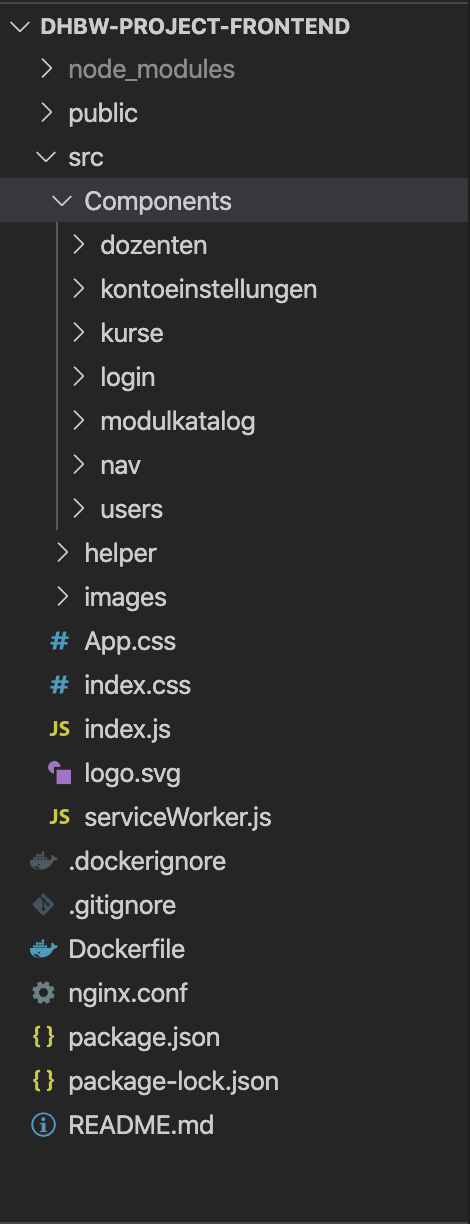
\includegraphics[scale=0.6]{img/FrontEnd/front-end-ordnerstruktur}
	\caption[Übersicht der Ordnerstruktur des Front-Ends]{\label{fig:Front-End_Ordnerstruktur}Übersicht der Ordnerstruktur des Front-Ends\footnotemark}
\end{figure}
\footnotetext{Verwendete Entwicklungsumgebung: Visual Studio Code (\url{https://code.visualstudio.com})}

%Darüber hinaus sind in React insbesondere die Konzepte \textit{Properties}, zu Deutsch Eigenschaften, und der \textit{State}, zu Deutsch Zustand. 
%Mithilfe von \textit{Properties} können Komponenten Informationen austauschen, sodass beispielsweise eine Eltern-Komponente relevante Informationen an eine Kind-Komponente weitergibt. 
%Die übergebenen Werte der Properties können jedoch nicht geändert werden. 
%
%Dementgegen können sich die Werte bei dem Konzept \textit{State} ändern. 
%Zu jeder Komponente gibt es einen Objekt-Zustand, \texttt{this.state}, worauf nur die Komponente selbst zugreifen und den Wert ändern kann. 
%Der State einer Komponente enthält Eigenschaften, die von der Komponente beobachtet werden können. 
%Wenn sich der State einer Komponente ändert, wird der \ac{DOM} angepasst und die Komponente mit den aktualisierten Werten gerendert. 

Sobald Änderungen in der Webanwendung vorgenommen werden, wird bei React nicht der komplette Seiteninhalt angepasst, sondern lediglich die tatsächlichen Veränderungen bei dem entsprechenden \ac{DOM}-Element angepasst. 
Der Vorteil hierbei ist, dass die Benutzeroberfläche schneller auf Veränderungen reagieren kann. 

Für eine einfachere Webentwicklung in React wurde \textit{Material-UI}\footnote{\url{https://material-ui.com}} verwendet. 
Material-UI ist ein Open-Source-Framework, das React Komponenten bereitstellt und dadurch eine schnelle Entwicklung ermöglicht.
Ein einheitliches Design System für React und die vielen nützlichen UI-Komponenten waren ausschlaggebend für die Entscheidung für Material-UI.

Entsprechend dem Design Entwurf aus Kapitel \vref{ch:DesignEntwurf} wurden die Komponenten so zusammengesetzt, dass sich der Seitenaufbau aus den Hauptkomponenten Kopfzeile, Navigationsleiste und Seiteninhalte zusammensetzt. 
In Abbildung \vref{fig:SeitenaufbauUmsetzung} ist die Umsetzung entsprechend dem Design Entwurf abgebildet.

\begin{figure}[h]
	\centering 	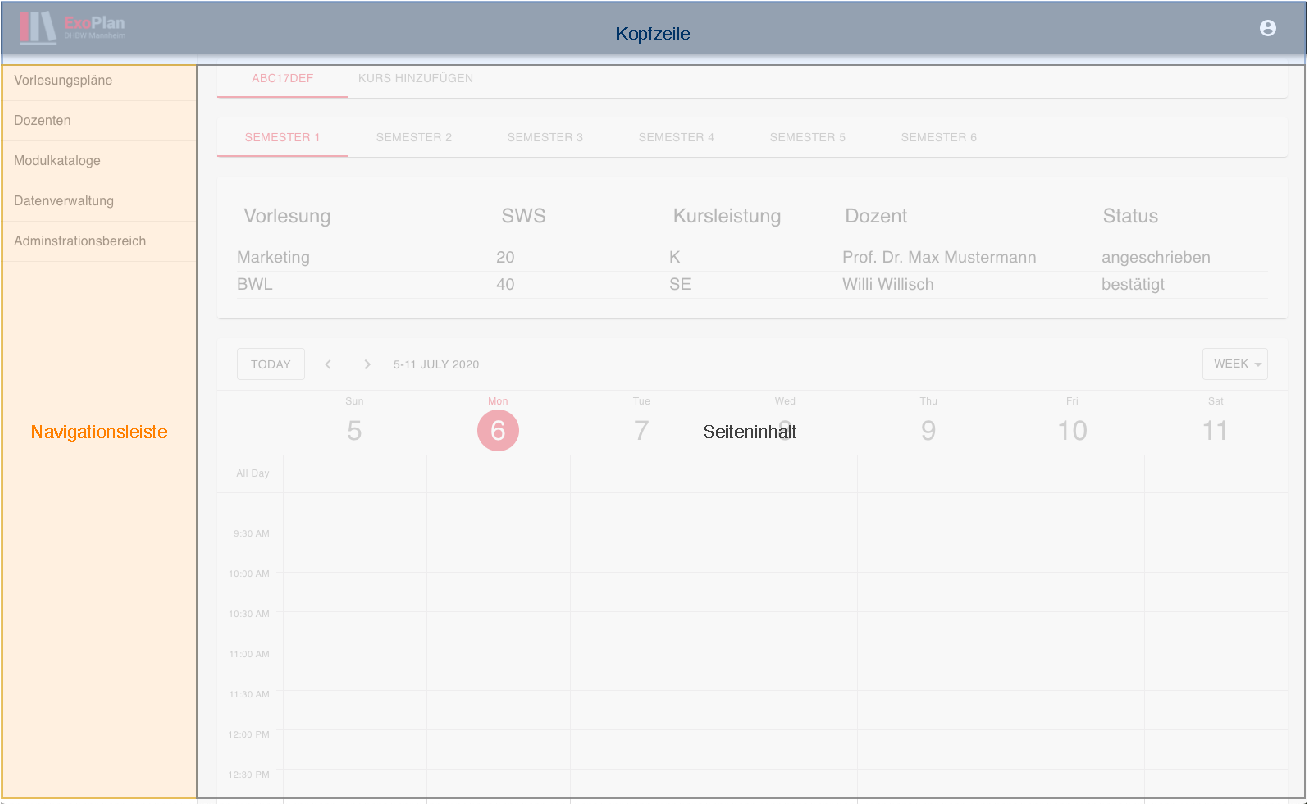
\includegraphics[width=\textwidth]{img/FrontEnd/UmsetzungDesign.pdf}
	\captionsetup{format=hang}
	\caption[Umsetzung der Benutzeroberfläche]{\label{fig:SeitenaufbauUmsetzung}Umsetzung der Benutzeroberfläche}
\end{figure}

\subsection{Styleguide für die Umsetzung}
Für ein einheitliches Erscheinungsbild der Webanwendung wurde in einem Styleguide definiert, welche Gestaltungsrichtlinen für die Entwicklung des Front-Ends gelten. 
Der Guide wurde den Front-End-Entwicklern zur Verfügung gestellt, damit 
sie diesen bei ihrer Entwicklung berücksichtigen können. 
In Abbildung \vref{fig:FE-StyleguideLogo} und \vref{fig:FE-StyColor} ist ein Auszug des Styleguides hinsichtlich des Logos und den einheitlichen Farben abgebildet.
Der vollständige Styleguide ist in Anhang \vref{an:Styleguide} einzusehen.
\begin{figure}[H]
	\centering 
	
\includegraphics[width=10cm]{img/FrontEnd/StyLogo.png}
	\caption[Auszug Styleguide für das Logo]{\label{fig:FE-StyleguideLogo}Auszug Styleguide für das Logo}
\end{figure}

\begin{figure}[H]
	\centering 
	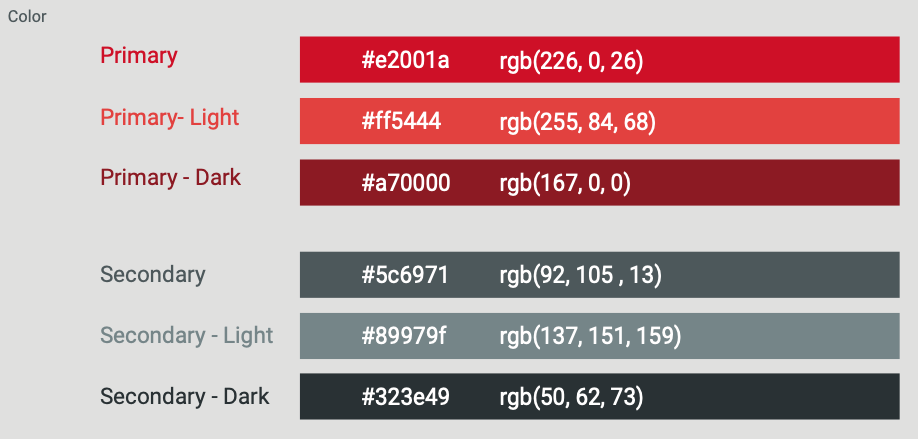
\includegraphics[width=10cm]{img/FrontEnd/StyColor.png}
	\caption[Auszug Styleguide für das Farbdesign]{\label{fig:FE-StyColor}Auszug Styleguide für das Farbdesign}
\end{figure}

\newpage
\subsection{Login}
Die Webanwendung startet gemäß der Anforderung A4 aus Tabelle \vref{anf:Profilzuordnung} mit einem Login, sodass sich der Benutzer anmelden oder registrieren kann. 
In Abbildung \vref{fig:FE-Login} ist die Login-Seite der Software zu sehen.
%Bei der Gestaltung der Seite wurde insbesondere auf die 
\begin{figure}[H]
	\centering 
	\includegraphics[width=\textwidth]{img/FrontEnd/Login.png}
	\caption[Login]{\label{fig:FE-Login}Login}
\end{figure}

\subsection{Kursübersicht}
Die Hauptansicht der Webanwendung ist die in Abbildung \vref{fig:FE-Vorlesungskalender} dargestellte Seite.
Hier werden die unterschiedlichen Kurse mit den jeweiligen Semestern, den Vorlesungen und dem eingebunden Kurskalendar angezeigt. 
Es können bereits angelegte Kurse verwaltet sowie neue Kurse angelegt werden. 
Die jeweiligen Vorlesungen können geplant werden, indem der aktuelle Stand der Vorlesungsorganisation mit der entsprechenden Dozentensuche angelegt wird.
In Unterkapitel \vref{ch:GC} wird die Einbindung des Kalendars sowie die Verbindung mit dem Google Calendar näher erläutert, da dies eine zentrale Komponente des Front-Ends darstellt.
%TODO Bild erneuern GC
\begin{figure}[H]
	\centering 
	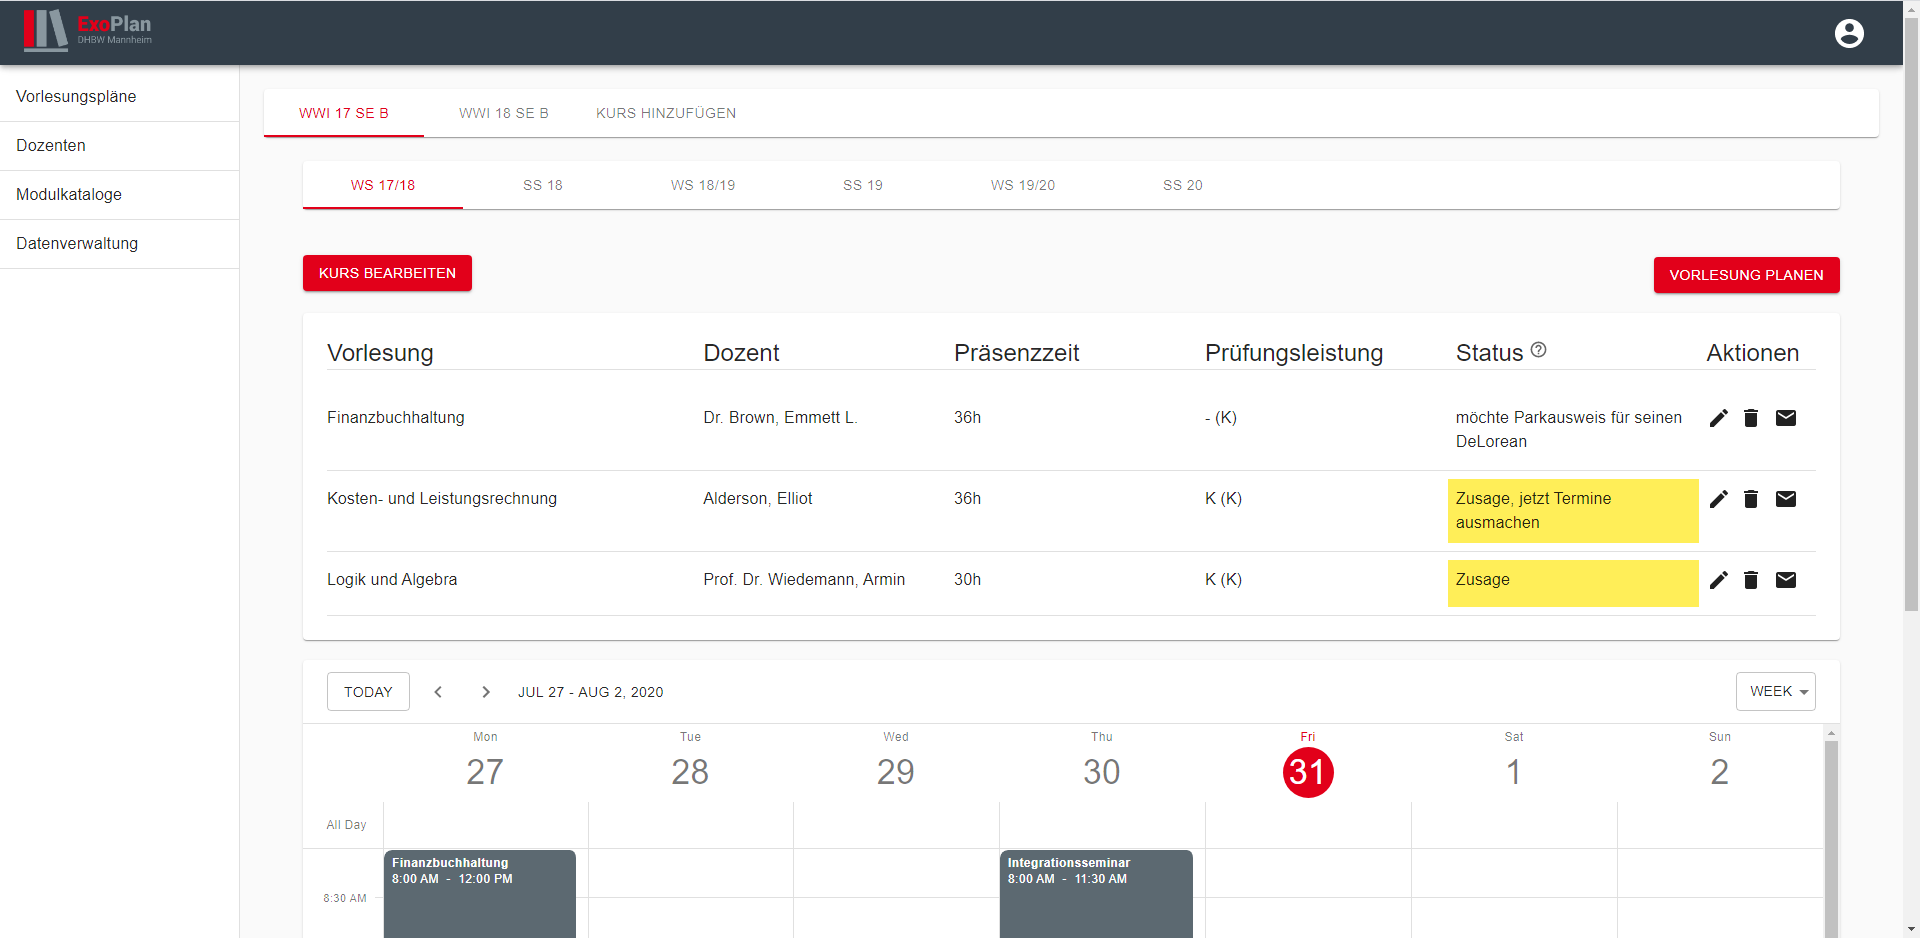
\includegraphics[width=\textwidth]{img/FrontEnd/Vorlesungskalender.png}
	\caption[Kursübersicht mit Vorlesungskalender]{\label{fig:FE-Vorlesungskalender}Kursübersicht mit Vorlesungskalender}
\end{figure}

\subsection{Dozentenansicht}
Unter dem Navigationspunkt \textit{Dozenten} wird der Dozentenpool dargestellt sowie die Möglichkeit zum Hinzufügen von neuen Dozenten gegeben.
Die Umsetzung der Anforderungen A1, A8, A9 und A12 aus Tabelle \vref{anf:Dozenten} ist in Abbildung \vref{fig:FE-Dozenten} zu sehen.
%In Abbildung \vref{fig:FE-DozentenDetail} ist 
Wird ein Dozent ausgewählt, erscheinen weitere Informationen in der Detail-Ansicht. Diese beinhaltet außerdem Funktionen, wie zum Beispiel das Hinterlegen eines Lebenslaufs.
\begin{figure}[H]
	\centering 
	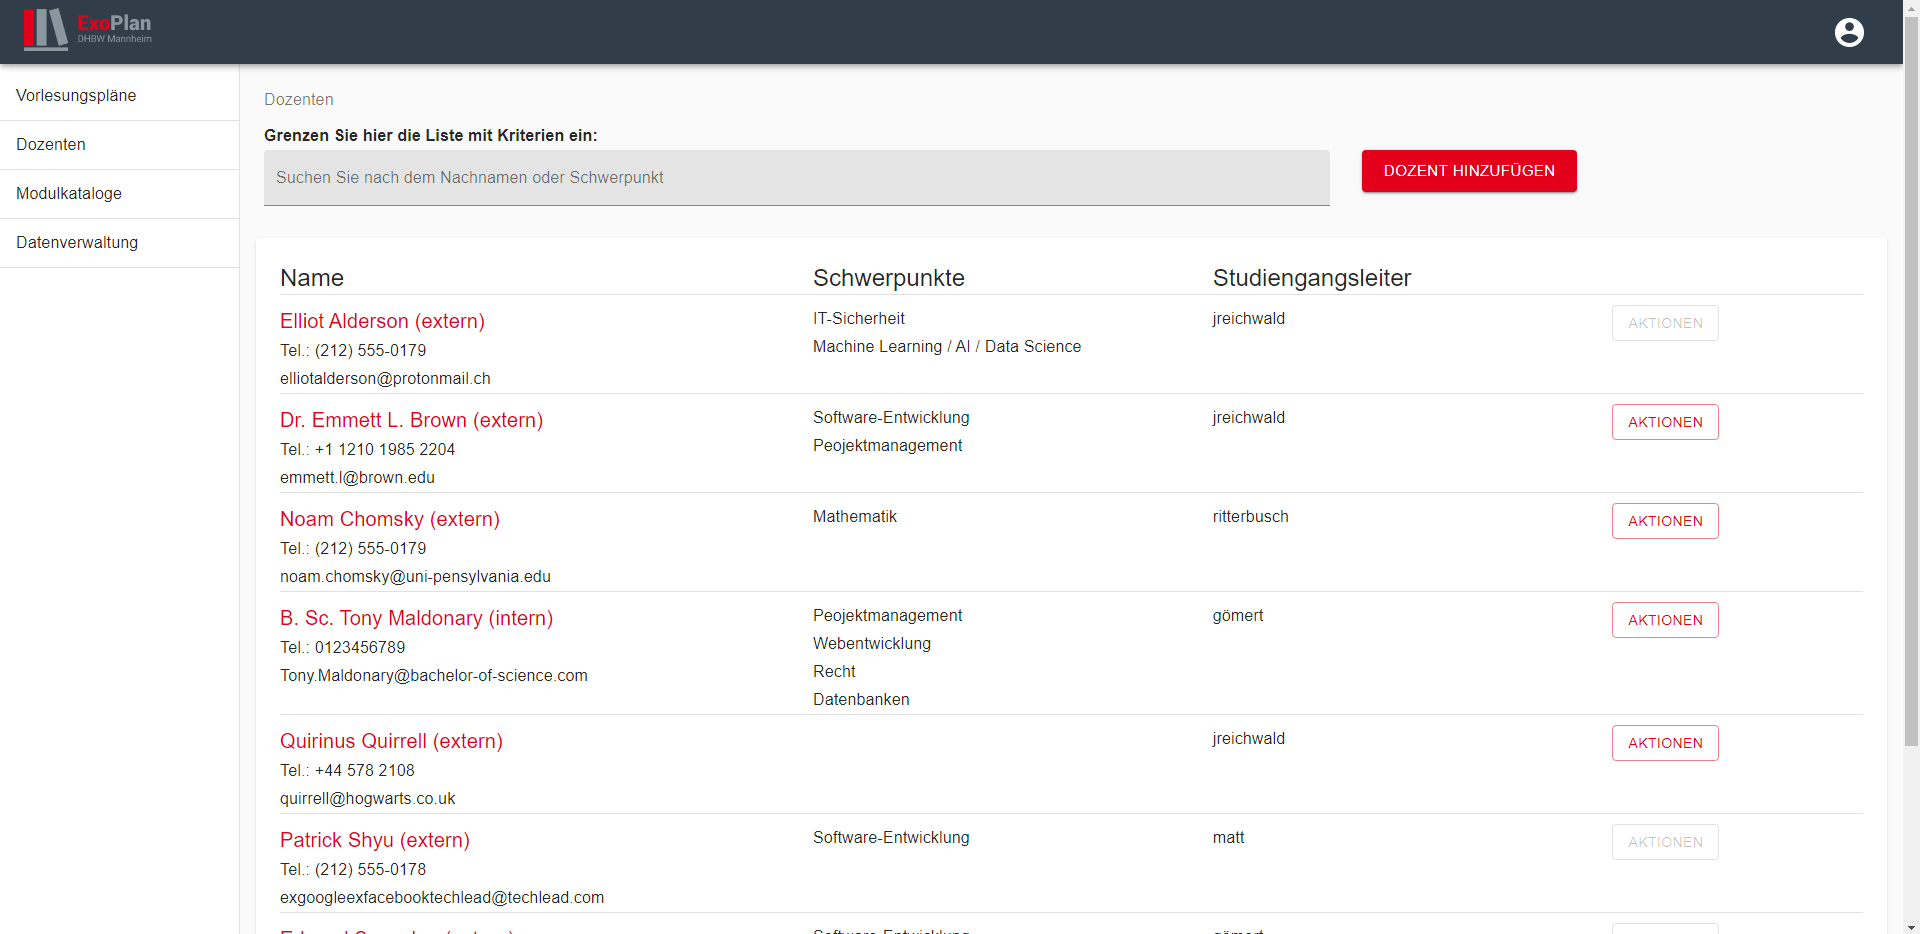
\includegraphics[width=\textwidth]{img/FrontEnd/Dozenten.png}
	\caption[Anzeige der Dozenten]{\label{fig:FE-Dozenten}Anzeige der Dozenten}
\end{figure}
%\begin{figure}[H]
%	\centering 
%	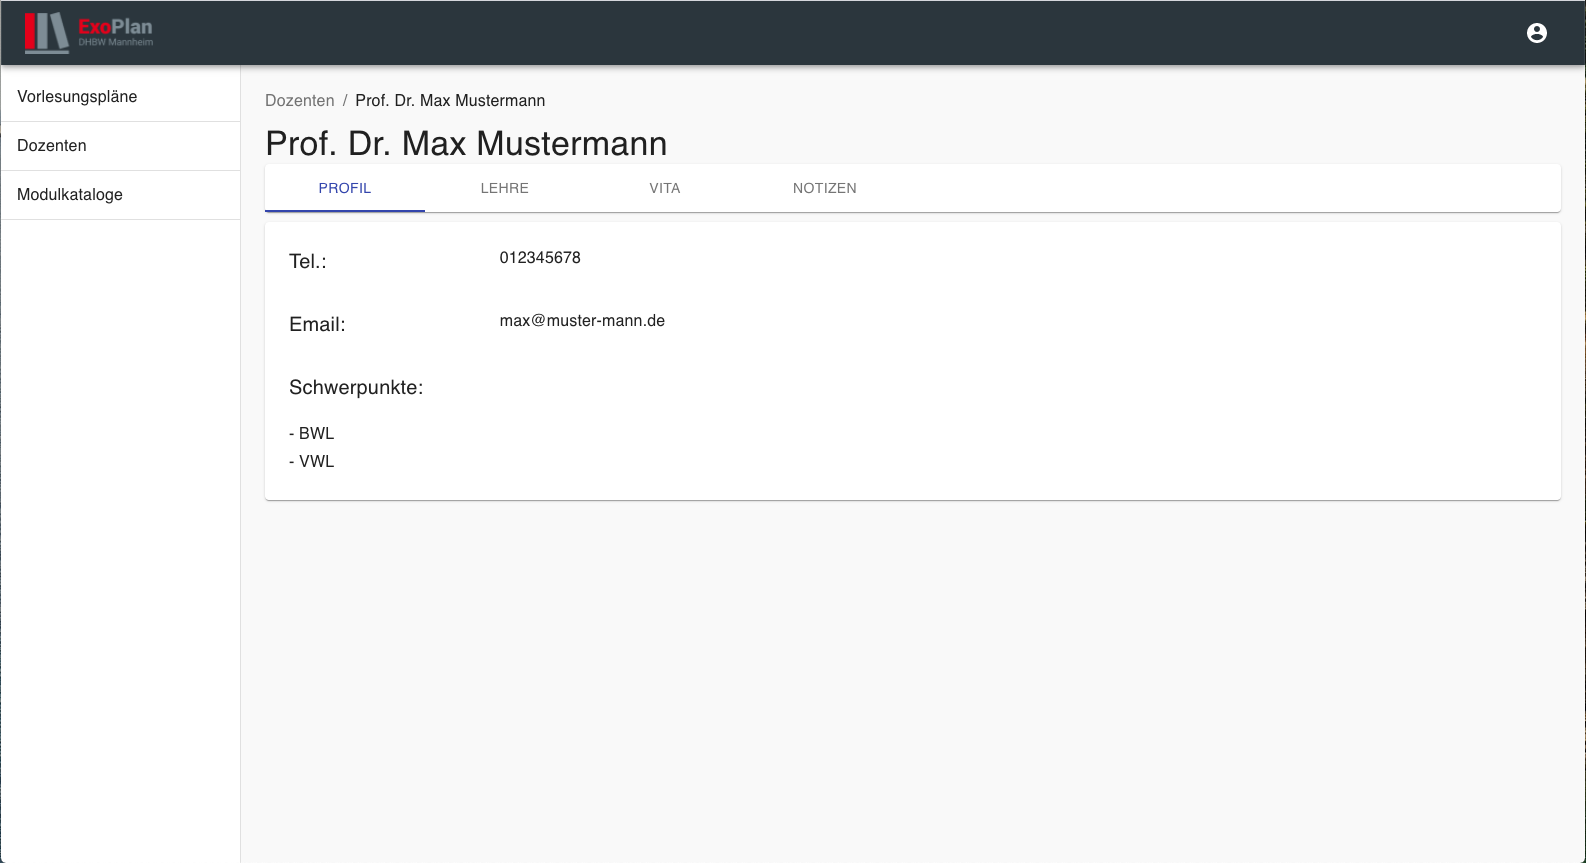
\includegraphics[width=\textwidth]{img/FrontEnd/DozentDetail.png}
%	\caption[Anzeige eines Dozenten]{\label{fig:FE-DozentenDetail}Anzeige eines Dozenten}
%\end{figure}

\subsection{Modulkatalog}
Mit dem Navigationspunkt \textit{Modulkatalog} wird die Anforderungen A4 aus Tabelle \vref{anf:Modulkatalog} umgesetzt. 
Es können Modulkataloge hinzugefügt, angezeigt sowie verwaltet werden. 
\begin{figure}[H]
	\centering 
	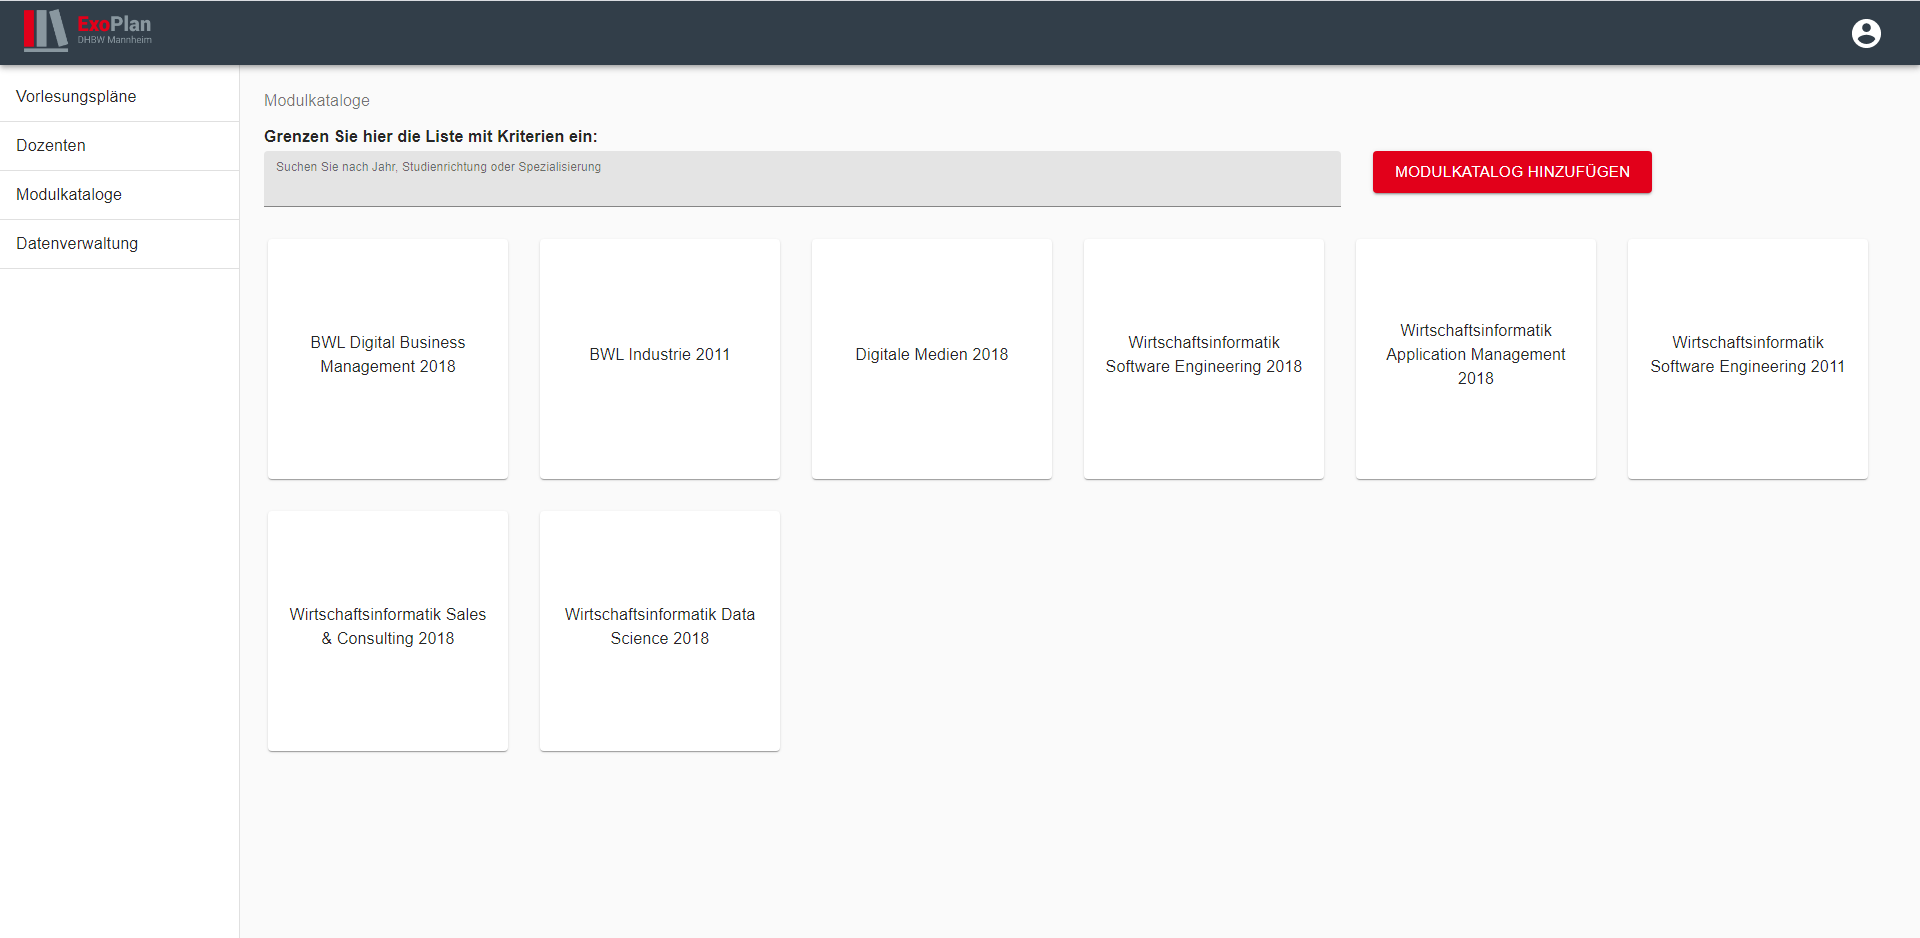
\includegraphics[width=\textwidth]{img/FrontEnd/Modulkataloge.png}
	\caption[Anzeige der Modulkatalogen]{\label{fig:FE-Modulkataloge}Anzeige der Modulkatalogen}
\end{figure}

\subsection{Datenverwaltung}
In der Datenverwaltung können die Studiengänge, die Schwerpunkte sowie die Prüfungsleistungen verwaltet werden.
In Abbildung \vref{fig:FE-Datenverwaltung} ist das Hinzufügen, Bearbeiten und Löschen von Studiengängen abgebildet.
\begin{figure}[H]
	\centering 
	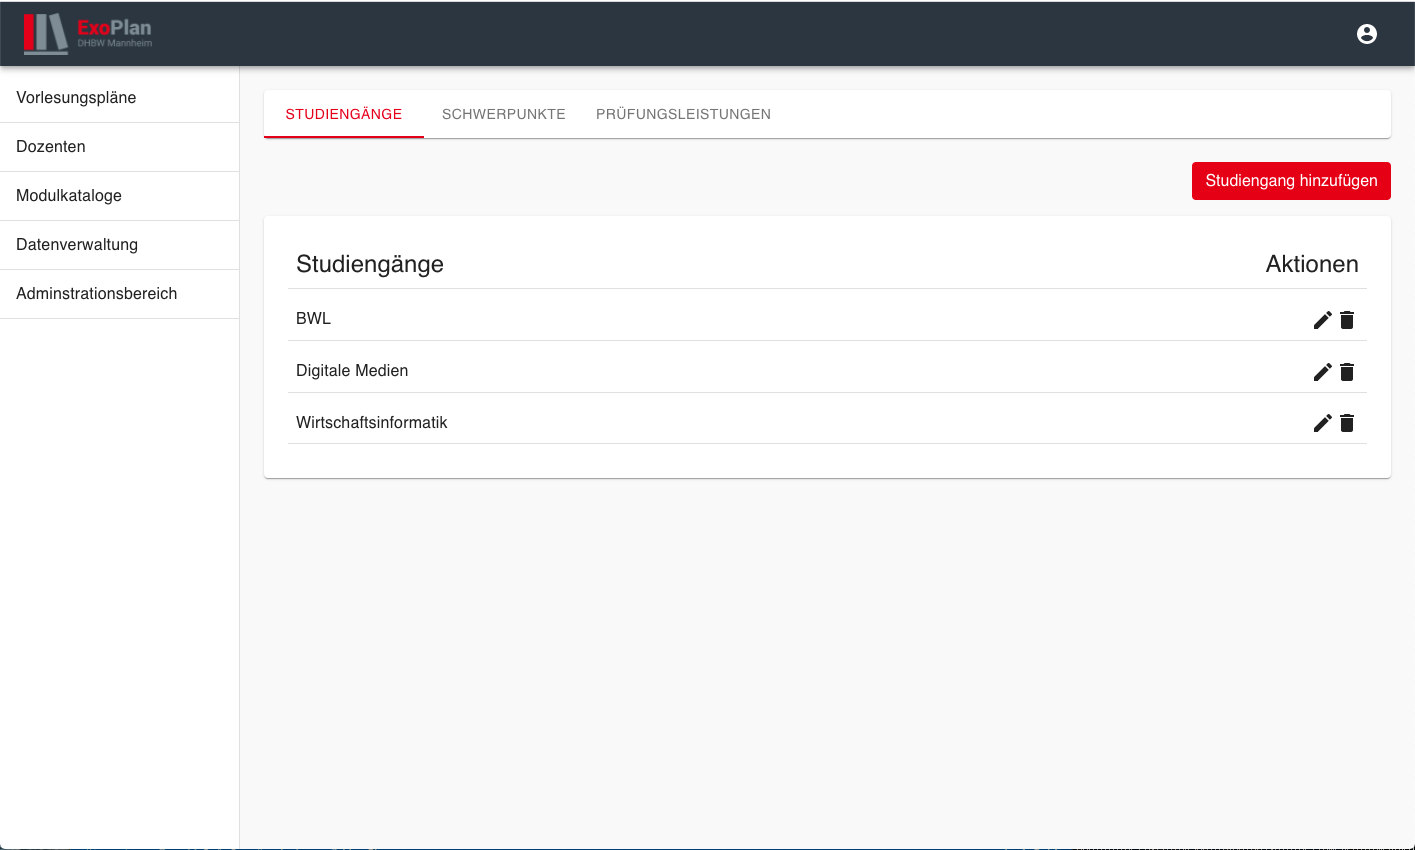
\includegraphics[width=\textwidth]{img/FrontEnd/Datenverwaltung.png}
	\caption[Datenverwaltung]{\label{fig:FE-Datenverwaltung}Datenverwaltung}
\end{figure}

\subsection{Administrationsbereich}
Der Administrationsbereich erlaubt es Nutzern mit der Benutzerart \textit{Administrator} andere Benutzer zu verwalten.
Neben dieser Funktionalität, in Abbildung \vref{fig:FE-Administrationsbereich} dargestellt, können Registrierungsschlüssel sowie der Zugang zu dem Google Calendar verwaltet werden.
\begin{figure}[H]
	\centering 
	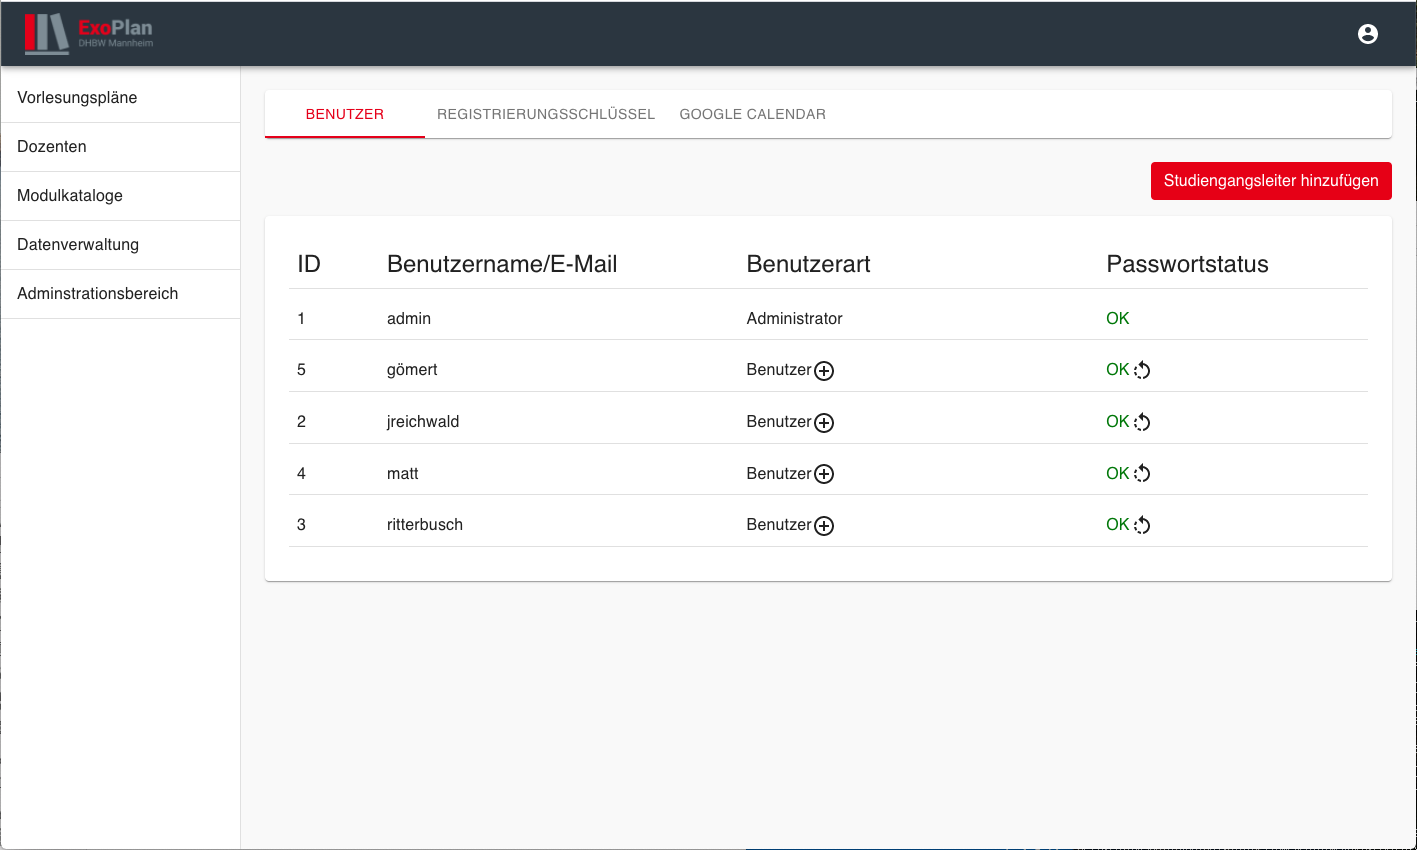
\includegraphics[width=\textwidth]{img/FrontEnd/Administrationsbereich.png}
	\caption[Administrationsbereich]{\label{fig:FE-Administrationsbereich}Administrationsbereich}
\end{figure}

\subsection{Allgemeine Einstellungen}
Zusätzlich können allgemeine Einstellungen für den Benutzer des Profils verändert werden, die in Abbildung \vref{fig:FE-Einstellungen} dargestellt sind.
So kann der Benutzer unter anderem sein Passwort ändern.
\begin{figure}[H]
	\centering 
	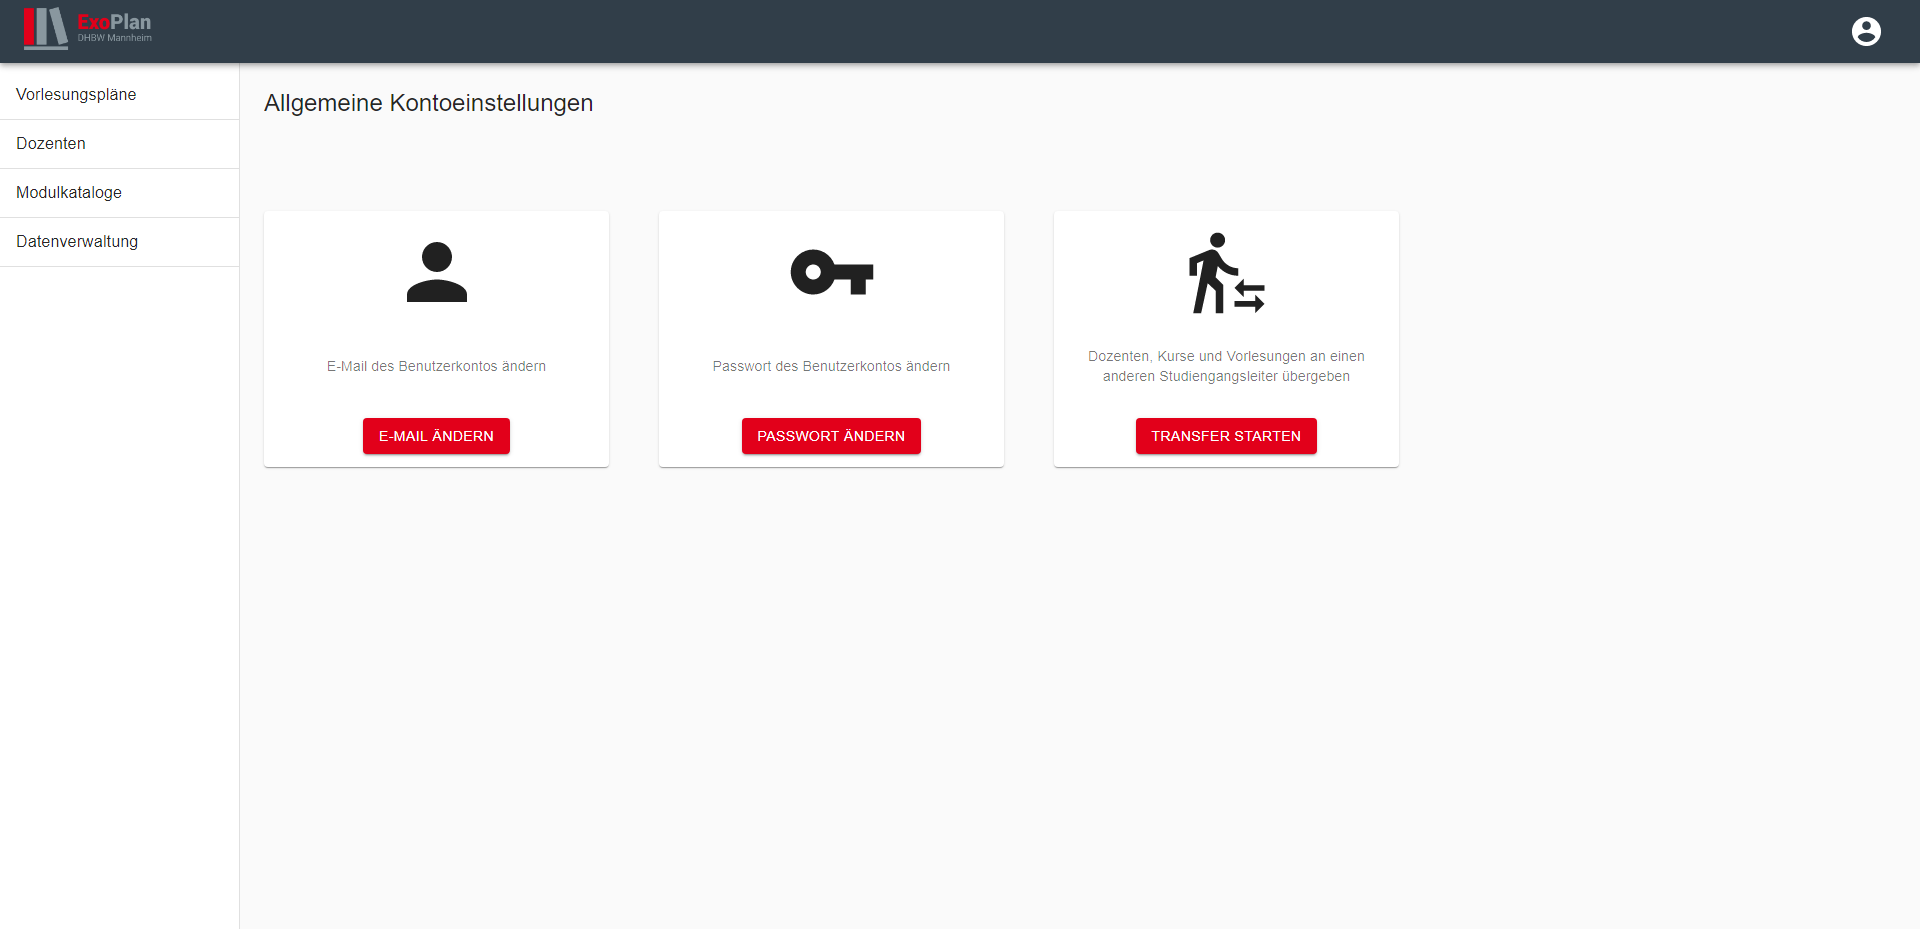
\includegraphics[width=\textwidth]{img/FrontEnd/Einstellungen.png}
	\caption[Allgemeine Kontoeinstellungen]{\label{fig:FE-Einstellungen}Allgemeine Kontoeinstellungen}
\end{figure}

\subsection{Vorlesungskalender mit Google Calendar}\label{ch:GC}
Damit der Studiengangsleiter die Vorlesungen organisieren kann, wird der Google Calendar gemäß der Anforderung A2 und A3 aus der Tabelle \ref{anf:GC} vollständig in die Software integriert.
Damit die Ereignisse der jeweiligen Google Calendar angezeigt sowie verwaltet werden können, muss ein Kalender in React implementiert werden. 

\subsubsection{Einbindung des DevExtreme React Scheduler}
Der \textit{DevExtreme React Scheduler}\footnote{\url{https://devexpress.github.io/devextreme-reactive/react/scheduler/}} ist eine Komponente für Material-UI, die einen Kalender für React bereitstellt. 
Das Erscheinungsbild des React Schedulers ist von dem Google Calendar inspiriert und benutzerfreundlich gestaltet.\autocite[Vgl.][]{ReactScheduler} 
Neben Funktionalitäten, wie beispielsweise Drag-and-Drop-Operationen sowie unterschiedlichen Anzeigeoptionen, ist insbesondere die Anbindung und Integration eines Google Calendars über geeignete Schnittstellen ausschlaggebend für die Entscheidung zur Verwendung der Komponente. 

In Abbildung \vref{fig:ReactScheduler} ist eine Übersicht mit erklärenden Ergänzungen über den implementierten und konfigurierten React Scheduler dargestellt. 
Zur Verwendung des React Schedulers wird ein Package und entsprechende Abhängigkeiten von NPM eingebunden.\footnote{\url{https://www.npmjs.com/package/@devexpress/dx-react-scheduler}}
Weitere Informationen zur Einbindung sowie Konfiguration des Kalenders sind in der Dokumentation von DevExtreme gegeben.\footnote{\url{https://devexpress.github.io/devextreme-reactive/react/scheduler/docs/guides/getting-started/}}
\begin{figure}[H]
	\centering 
	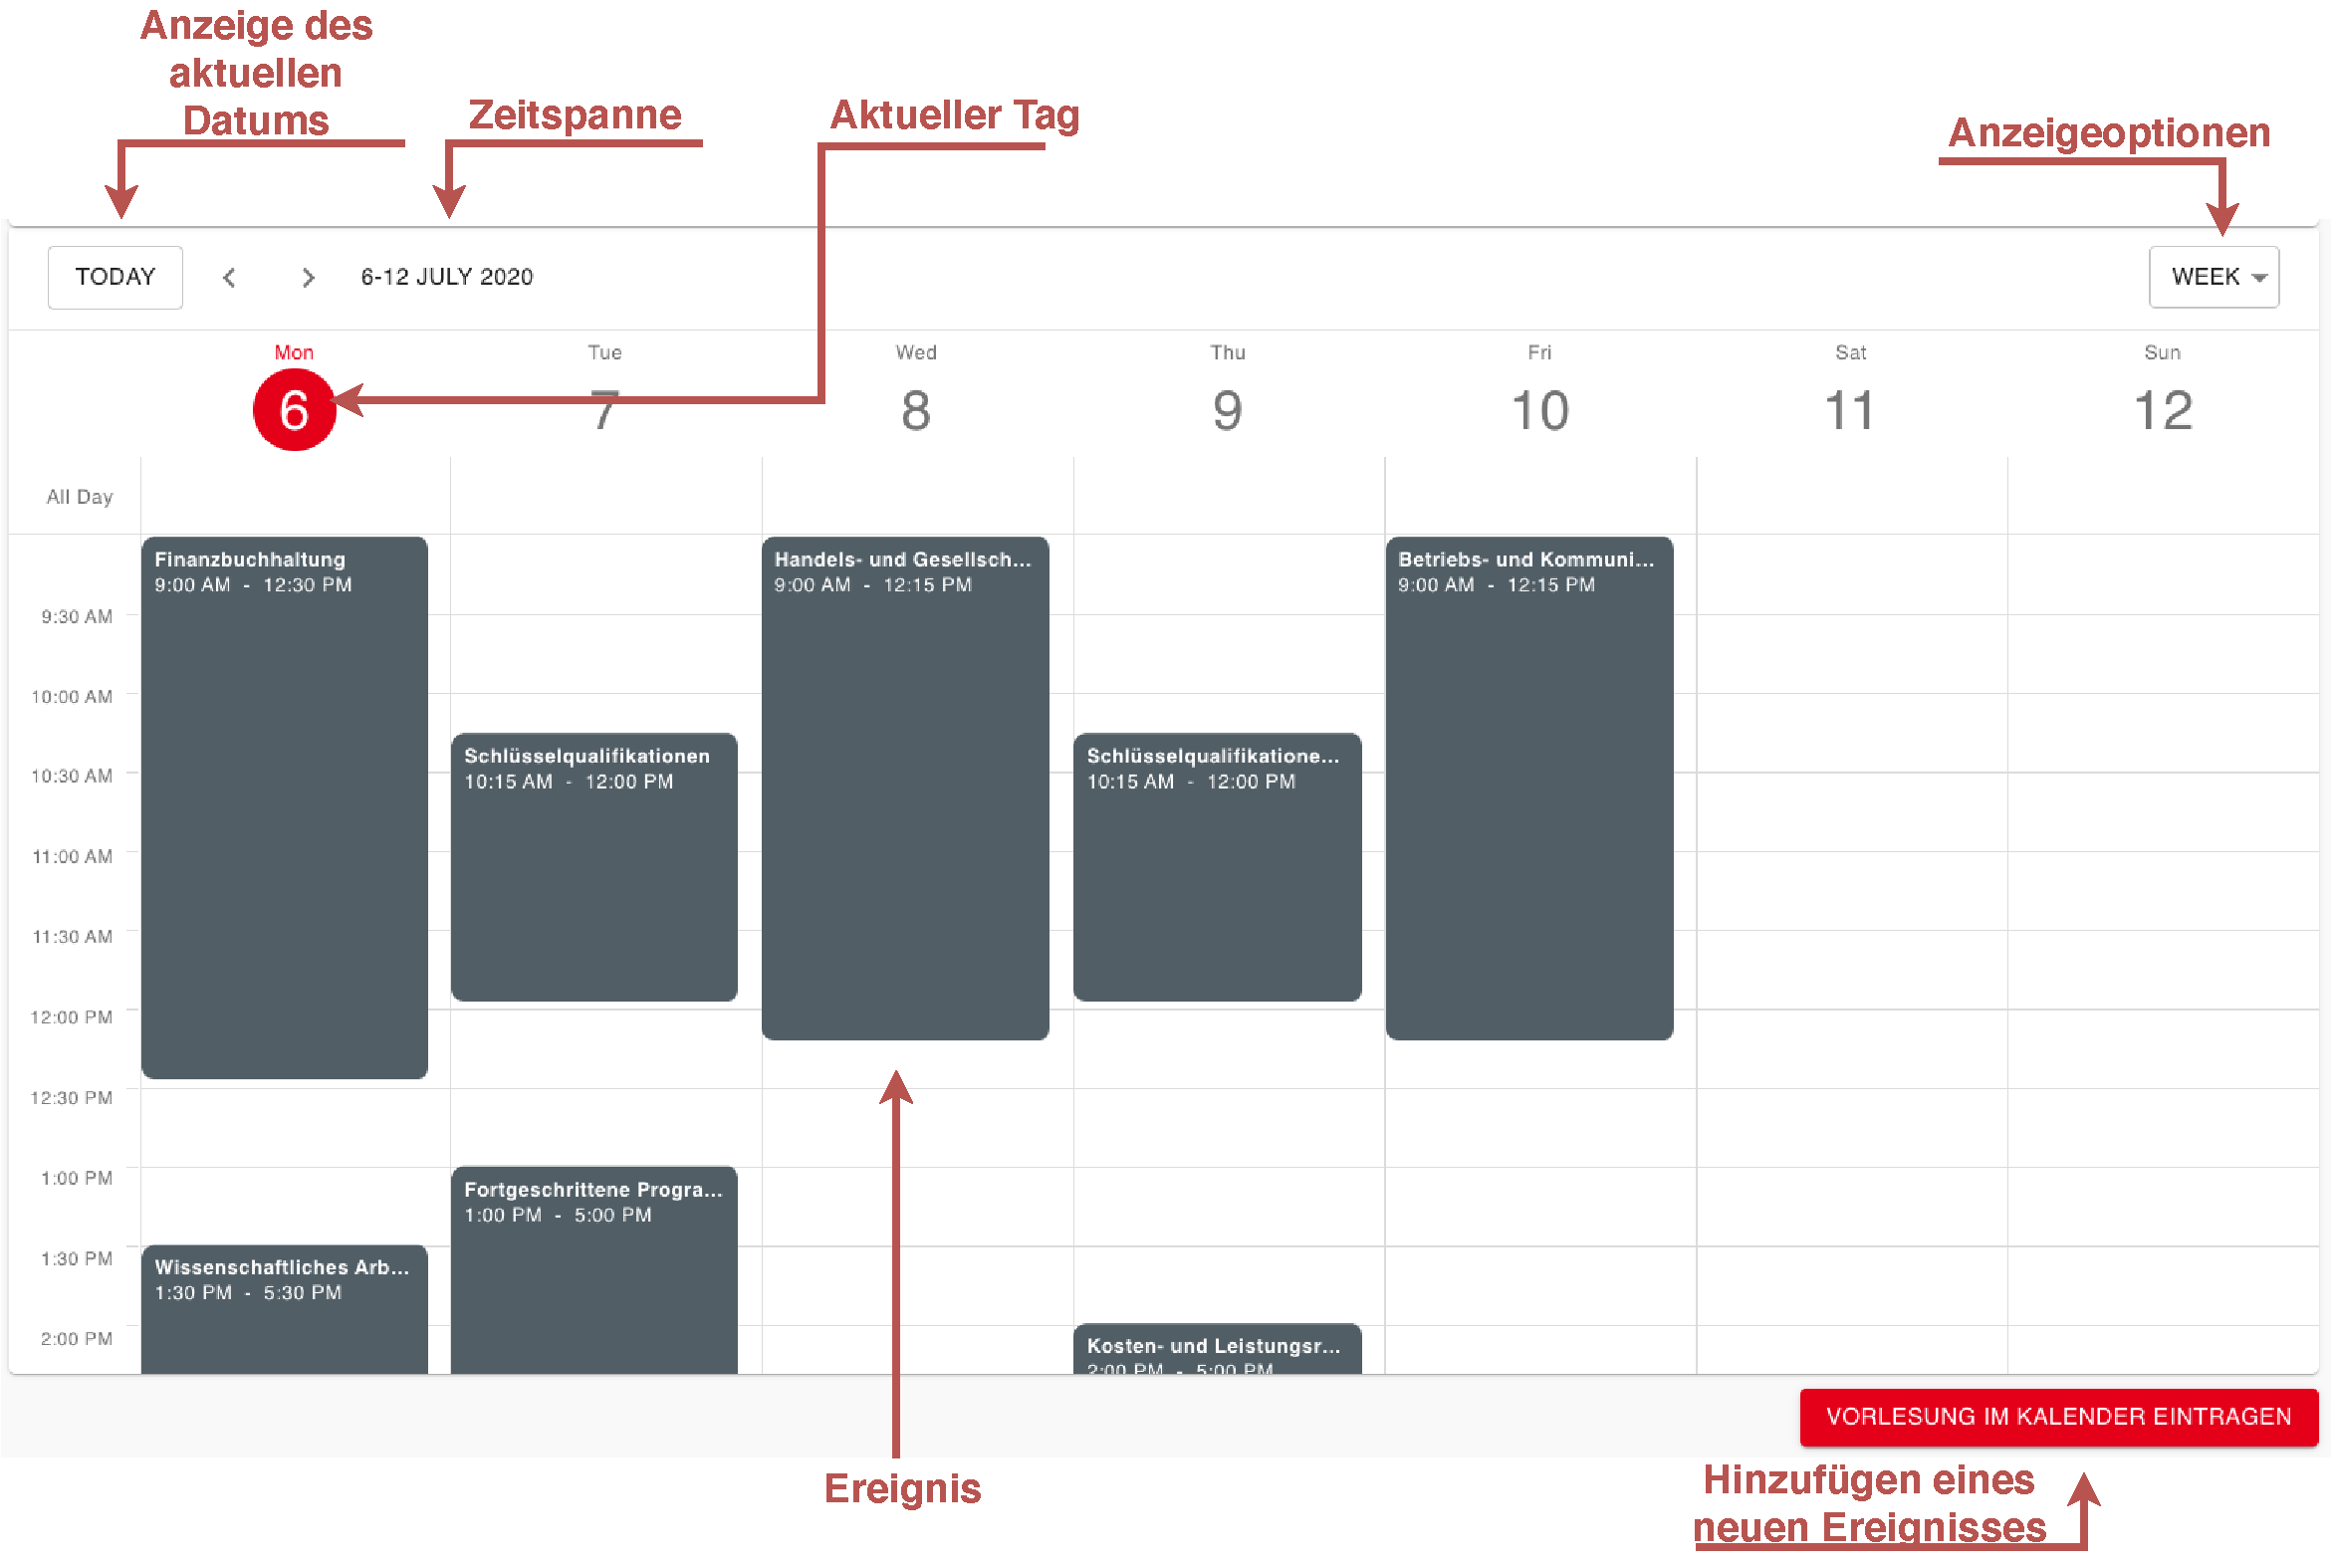
\includegraphics[width=\textwidth]{img/FrontEnd/ReactCalendar.pdf}
	\caption[Übersicht des React Schedulers]{\label{fig:ReactScheduler}Übersicht des React Schedulers}
\end{figure}

\subsubsection{Initialisierung und Verbindung des Google Calendars}
Der Google Calendar ermöglicht eine Anbindung an das System über eine \ac{API}.
Damit die Inhalte eines Google Calendars über die Google Calendar-\ac{API}-Schnittstelle\footnote{\url{https://developers.google.com/calendar/v3/reference}} angefragt und in dem React Scheduler angezeigt werden können, müssen die Anfragen über einen Token authentifiziert werden. 
Hierfür wird OAuth 2.0 verwendet, um die Authentifizierung durchzuführen.\autocite[Vgl.][]{GCApi} 

In der JavaScript-Datei \texttt{apiHandlerGoogleCalendar.js} sind die Funktionalitäten für die Kommunikation zwischen Google Calendar-\ac{API} und der Webanwendung implementiert. 
Der notwendige \ac{API}-Key und die Information bezüglich des OAuth-Client-IDs werden im Administrationsbereich unter dem Tab \textit{Google Calendar} abgelegt. 
Der \ac{API}-Key und die OAuth-Client-ID werden vor jedem Aufruf des Google Calendars aus dem Back-End abgerufen. 
Diese werden zusammen mit der Google Calendar-ID bei den Anfragen mitgegeben. 
Beim Erstmaligen Einloggen mit einem Google-Account wird die Login-Session gespeichert und hinterlegt. 
Mit einem validen \ac{API}-Key und der Berechtigung zum Bearbeiten werden die Anfragen an die Google Calendar-\ac{API} genehmigt und die Inhalte des jeweiligen Kalenders an die Anwendung übertragen.
Die erhaltenen Inhalte werden formatiert und in dem React Scheduler angezeigt.

\subsubsection{Interaktion mit dem Kalender}\label{ch:InteraktionGC}
Zur Funktionalität des Kalenders werden drei unterschiedliche Interaktionen mit dem Google Calendar benötigt: das Hinzufügen, das Ändern sowie das Löschen von Ereignissen. Im Folgenden werden die Anfragen an die \ac{REST}-\ac{API} des Google Calendars näher beschrieben.

\textbf{Anzeigen von Ereignissen}\newline
In dem React Scheduler können Ereignisse aus dem Google Kalender angezeigt werden.
Diese Funktion wird benötigt, damit der Google Calendar und der DevExtreme React Scheduler den gleichen Stand besitzen.
Sonst könnte es bei fehlgeschlagenen Aktionen zu Inkonsistenzen kommen.

\textbf{Hinzufügen von Ereignissen}\newline
In dem React Scheduler können neue Ereignisse dem Kalender hinzugefügt werden.
In Abbildung \vref{fig:AddReactScheduler} ist das Dialog-Fenster abgebildet, welches nach dem Drücken des Hinzufügebuttons erscheint.
\begin{figure}[H]
	\centering 
	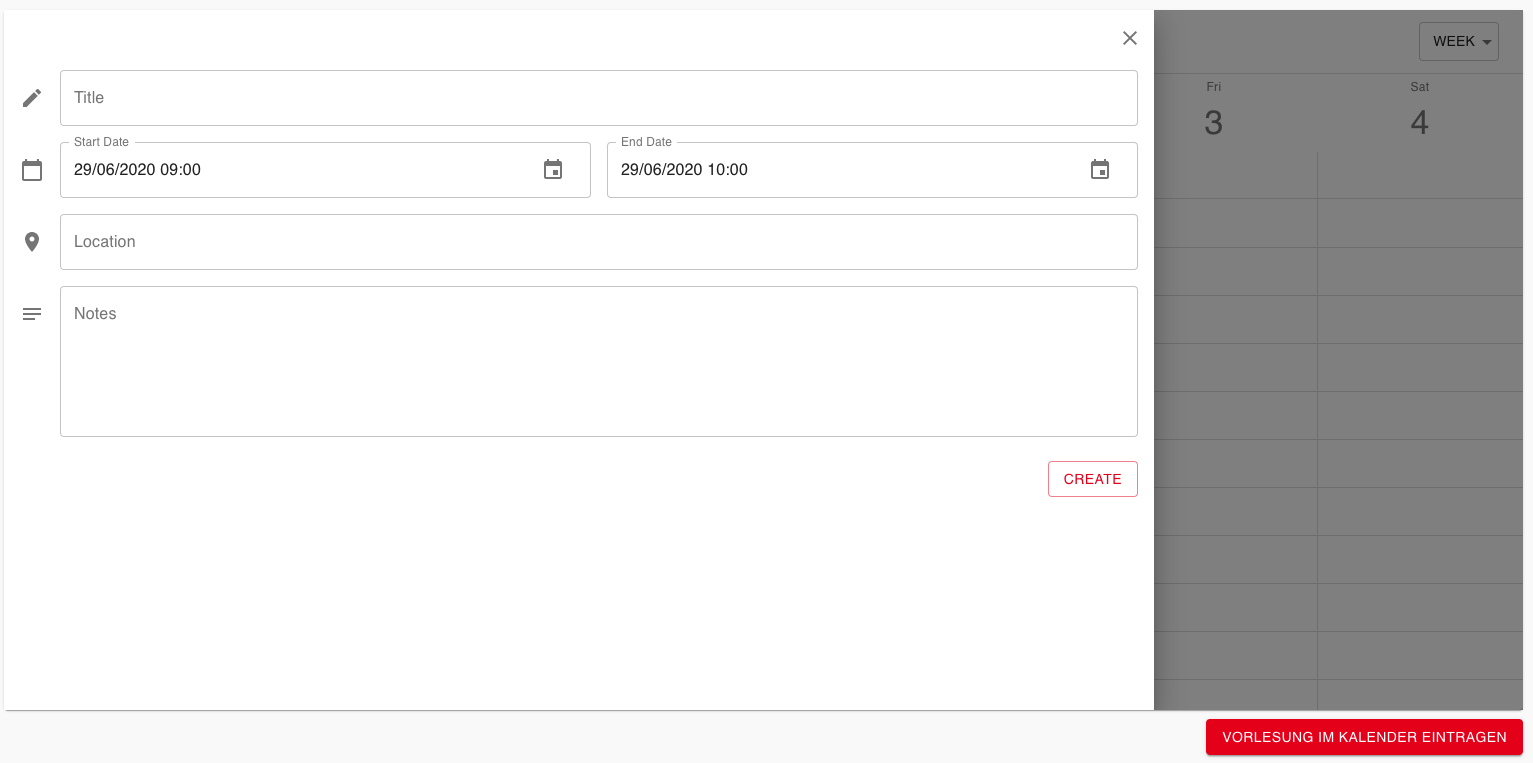
\includegraphics[width=\textwidth]{img/FrontEnd/GCAdd.png}
	\caption[Erstellen eines Ereignisses im React Scheduler]{\label{fig:AddReactScheduler}Erstellen eines Ereignisses im React Scheduler}
\end{figure}

Zusätzlich zu den abgebildeten Inhalten werden die Kalender-ID und der Token bei der PUSH-Anfrage übermittelt. Hierbei wird die Bibliothek \textit{GAPI} von Google verwendet, die eine einfache Verbindung mit der \ac{API} über browserseitiges JavaScript ermöglicht. 
Eine detaillierte Dokumentation dieser Anfrage ist in der Schnittstellenbeschreibung der Google Calendar \ac{API} gegeben.\footnote{\url{https://developers.google.com/calendar/v3/reference/events/insert}}

\textbf{Ändern von Ereignisssen}\newline
Vorhandene Ereignisse können ebenfalls bearbeitet werden, indem die entsprechende Veranstaltung ausgewält und der Bearbeiten-Button auf dem erscheinenden Popup geklickt wird, welches in Abbildung \vref{fig:GCPopup} dargestellt ist. 
\begin{figure}[H]
	\centering 
	
\includegraphics[width=6cm]{img/FrontEnd/GCPopup.png}
	\caption[Popup eines Ereignisses im React Scheduler]{\label{fig:GCPopup}Popup eines Ereignisses im React Scheduler}
\end{figure}

Zur Änderung der Daten wird eine \ac{API}-Anfrage mit der Methode \textit{update} verwendet.\footnote{\url{https://developers.google.com/calendar/v3/reference/events/update}} 
Diese ist vom Aufbau ähnlich zu der zuvor vorgestellten \textit{insert}-Methode.

\textbf{Löschen von Ereignissen}\newline
Zusätzlich können Ereignisse in dem Google Calendar gelöscht werden, indem die Funktionalität, ebenfalls in Abbildung \vref{fig:GCPopup} abgebildet, genutzt wird. 
Zur Durchführung dieser Operation wird das Event \textit{delete} verwendet, wobei lediglich die Calendar-ID sowie die Event-ID übermittelt werden.\footnote{\url{https://developers.google.com/calendar/v3/reference/events/delete}}   
In dem Code-Ausschnitt \vref{lst:deleteEvent} ist die Erstellung der Delete-Anfrage abgebildet.

\lstset{language=JavaScript}
\begin{lstlisting}[caption={Anfrage zum Löschen eines Ereignisses}, label={lst:deleteEvent}]
function handleAppointmentDelete(deleteAppointmentId, gapi) {
  var request = gapi.client.calendar.events.delete({
    'calendarId': gcID,
    'eventId': deleteAppointmentId
  });

  request.execute(function (response) {
    if (response.error || response === false) {
      showSnackbar('Loeschen fehlgeschlagen. 
      Neuladen der Seite erforderlich.', SEVERITY.ERROR);
    } else {
      showSnackbar('Vorlesung erfolgreich geloescht.',
      SEVERITY.SUCCESS);
    }
  });
}
\end{lstlisting}


\section{Verknüpfung Backend und Frontend}

\section{Zugriffsberechtigungen}
\section{Test}
Aufgrund der begrenzten Zeit wurde während der Entwicklung hauptsächlich manuell getestet. 
Als weitere Maßnahme zur Qualitätssicherung werden Code Reviews eingesetzt.
Neben Pair Programming sowie Walkthroughs werden hauptsächlich tool-basierte Code Reviews genutzt, indem bei GitHub per Pull Request Feedback von geeigneten anderen Entwicklern zu jeder Codeänderung eingefordert wird.
Dadurch kann die Codequalität sichergestellt sowie Feedback zu den Funktionalitäten eingeholt werden.

Nach Beendigung der Entwicklung wurde außerdem im Front-End ein Abnahmetest von dem Projektergebnis durchgeführt, um die Funktionalitäten zu prüfen sowie einen Abgleich der Benutzeroberfläche durchzuführen. 
Hierbei wurde die Referenzen Design Entwurf aus Kapitel \vref{ch:DesignEntwurf}, der Styleguide im Anhang \vref{an:Styleguide} sowie die Anforderungen der Tabelle \vref{tab:Anforderungen} hinzugezogen.
Dabei wurden mehrere geringfüge Fehler gefunden sowie direkt verbessert. 
Zusätzlich wurden Aspekte festgehalten, die zeitlich nicht mehr geändert sowie umgesetzt werden können, jedoch aber für eine Weiterentwicklung des Produkts von Relevanz sind: 

\begin{itemize}
    \item Erlaubte Formate und maximale Dateigröße von hochgeladenen Dokumenten
    \item Löschen von Modulkatalogen 
    \item Entziehen von Administrationsrechten
    \item Studiengangsrichtung nur bei zutreffenden Studiengängen anzeigen (z.B. der Studiengang Digitale Medien hat keine Studienrichtungen)
    \item Hinzufügen von Vorlesungsinformationen zu den Kalendareinträgen.
\end{itemize}
\chapter{User Guide}

\section{Setup}
\begin{itemize}
	\item Wie bekommt man das Projekt? / Woraus besteht das Paket?
	\item Was muss man tun, um die Web-Anwendung aufzusetzen? 
	\item Welche Konfigurationen müssen vorgenommen werden?
	\item Was sind die Login-Daten? 
	\item VM, Docker
\end{itemize}

\section{Funktionalitäten}
In diesem Abschnitt soll eine grobe Übersicht über die Hauptfunktionalitäten von ExoPlan gegeben werden. 
Diese sind nachfolgend aufgelistet und werden anschließend näher erklärt.

\begin{itemize}
	\item Neuen Kurs anlegen,
	\item Dozenten kontaktieren (Status nutzen),
	\item Vorlesungen im Kalender verwalten,
	\item Modulkatalog verwalten,
	\item Datenverwaltung - Studiengänge, Schwerpunkte, Prüfungsleistungen,
	\item Administration - Registrierungsschlüssel, Benutzer, Google-Calendar.
\end{itemize}

\subsection{Neuen Kurs anlegen}

Um einen neuen Kurs in ExoPlan anzulegen, muss sich der Benutzer mit seinen Anmeldedaten anmelden. 
Anschließend kann in der Anwendung auf der linken Seite der Menüpunkt \textit{Vorlesungspläne} ausgewählt werden. 
Daraufhin kann der Tab \textit{Kurs hinzufügen} geöffnet werden.

Damit das volle Potential des ExoPlan-Systems vollumfänglich ausgeschöpft werden kann, muss die Kurskonfiguration sehr genau durchgeführt werden. 
Hierbei wird zuerst der Name des Kurses angegeben, also zum Beispiel \textit{WWI17SEB}. 
Außerdem müssen Studiengang (beispielsweise Wirtschaftinformatik, BWL, usw.) und Studienrichtung (beispielsweise Software Engineering oder Sales and Consulting) für den Kurs spezifiziert werden. 
Abschließend wird die Anzahl der Semester ausgewählt, der Zeitraum für jedes Semester angegeben und die Google Calender-ID des Kurses eingetragen. 
Die Zeiträume der Semester werden anschließend mit den Modulkatalogen abgeglichen, wodurch später nur Vorlesungen zur Planung zur Verfügung stehen, welche auch durch den jeweiligen Modulkatalog im Gültigkeitszeitraum vorgesehen sind.

\subsection{Dozenten kontaktieren}

Im Studienalltag gilt es viele verschiedene Informationen gleichzeitig zu bewältigen. 
Ein großes Problem ist hierbei ein Überblick über die vorhandenen Dozenten und ihre Expertise zu behalten. 
Aus diesem Grund bietet ExoPlan eine leistungsstarke und zugleich einfache Dozentenverwaltung. 
Diese liefert Kontaktdaten, Informationen zu Qualifikationen und Auskunft darüber, welchem Studiengangsleiter ein Dozent zugeordnet ist.

Auch neue Dozenten können durch den Button \textit{Dozent hinzufügen} zu ExoPlan hinzugefügt werden.
\subsection{Vorlesungen im Kalender verwalten}

Das Planen von Vorlesungen und die Verwaltung dieser im Kalender des Kurses, ist eine grundlegende Funktionalität von ExoPlan. 
Hierzu wird im Menü auf der rechten Seite der Menüpunkt \textit{Vorlesungspläne} ausgewählt. 
Anschließend erhält man eine Übersicht zu den vorhandenen Kursen. 
Um eine Vorlesung für einen bestimmten Kurs zu planen, wird der betreffende Kurs-Tab ausgewählt und über den Button \textit{Vorlesung planen} oder direkt im angezeigten Kalender eine neue Vorlesung hinzugefügt. 
Wichtig zu beachten ist, dass die Vorlesungen vorher im dazugehörigen Modulkatalog erstellt wurde.

Damit der Kalender von Google importiert werden kann, müssen vorher die betreffenden Anmeldedaten eingegeben werden. 
Diese werden über ein Pop-Up-Fenster abgefragt. 
Wurden alle Daten korrekt eingegeben, wird der Google-Kalender des betreffenden Kurs in ExoPlan eingebunden und sychronisiert. 
Nun können einzelne Vorlesungstermin mit einem Klick auf den Button \textit{Vorlesung im Kalender eintragen} oder direkt in dem angezeigten Kalender hinzugefügt werden. 
Auch ein einfaches Verschieben der Termine über die Benutzeroberfläche ist möglich.

\subsection{Modulkatalog verwalten}

Zusätzlich lassen sich Modulkataloge in ExoPlan verwalten, speichern und anpassen. 
Diese bilden die Grundlage für die Planung von Vorlesungen und des gesamten Studienablaufs in ExoPlan. 
Dazu wird der Menüpunkt \textit{Modulkataloge} auf der linken Seite ausgewählt. 
Anschließend werden alle vorhandenen Modulkataloge angezeigt. 
Des Weiteren kann ein neuer Modulkatalog durch einen Klick auf den Button \textit{Modulkatalog Hinzufügen} erstellt werden. 

Ein Modulkatalog kann auch durch eine Auswahl geöffnet werden. 
Hierbei werden anschließen alle dazugehörenden Module angezeigt. 
Die einzelnen Module lassen sich bearbeiten sowie löschen.

\subsection{Datenverwaltung}

In der Datenverwaltung können die Studiengänge, Schwerpunkte von Dozenten sowie Prüfungsleistungen verwaltet werden.
Diese können jeweils hinzugefügt, bearbeitet oder gelöscht werden, damit diese in der Anwendung korrekt hinterlegt sind.

\subsection{Administrationsbereich}

Im Administrationsbereich können verschiedene Einstellungen vorgenommen werden, um den Betrieb von ExoPlan zu gewährleisten. 
Der Administrationsbereich kann durch den Menüpunkt \textit{Administrationsbereich} aufgerufen werden.

\subsubsection{Benutzerverwaltung}

Die Benutzerverwaltung kann über den Tab \textit{Benutzer} erreicht werden und liefert eine Übersicht über alle im System registrierten Benutzer. 
Es werden Informationen zur Art des Benutzers (Administrator, Studiengangsleiter und Benutzer) und der Passwortstatus (OK, Wechsel erforderlich) angegeben. 
Des Weiteren kann in dieser Übersicht ein Studiengangsleiter angelegt und auch ein Passwort-Reset durchgeführt werden.

\subsubsection{Registrierungschlüssel}

Registrierungsschlüssel werden benötigt, damit sich neue Benutzer in ExoPlan registrieren können. 
Dieser Schlüssel kann über den Tab \textit{Registrierungschlüssel} festgelegt werden.

\subsubsection{Google Calender}

In dieser Übersicht werden alle wichtigen Attribute zur Verwendung der Google-Calender-API konfiguriert:
\begin{itemize}
	\item Client-ID
	\item API-Key
	\item Client-Schlüssel.
\end{itemize}

\chapter{Evaluation}

\section{Bewertung Umsetzung}
\section{Lessons Learned}
Während der Arbeit an dem Projekt wurden viele Erkenntnisse gewonnen, neues Wissen erlangt sowie wertvolle Erfahrungen gesammelt.
Zunächst lässt sich festhalten, dass die Projektmitglieder viel technische als auch organisatorische Aspekte gelernt haben.
Im Folgenden werden drei Lessons Learned näher erläutert, die Optimierungspotenziale während oder nach dem Projekt bereitgehalten haben.
\subsection{Kommunikation}
Eine Herausforderung, die in jedem Gruppenprojekt zu meistern ist, ist die Kommunikation zwischen den Projektmitgliedern erfolgreich zu gestalten. 
Hierbei war eine besondere Hürde auch die Gruppengröße, die ein zusätzlicher Faktor für die Koordination und die Absprachen war. 
Ein respektvoller Umgang zwischen den Projektmitgliedern ist sehr wichtig und beeinflusst den Projektverlauf.
Während des Projektverlaufs wurde die Erkenntnis gezogen, dass eine verstärkte Kommunikation in den Teams sich positiv auf den Fortschritt auswirkt. 
Diese Optimierungsmöglichkeit wurde nach einer Reflexion des 5. Semesters gezogen und somit im 6. Semester verbessert. 

\subsection{Inhaltliche Ziele mit festen Milestones}
Wie bereits in der \hyperref[ch:zeitplanung]{Zeitplanung} ersichtlich, wurden in dem 6. Semester auch inhaltliche Ziele festgelegt. 
Diese Vorgehensweise hat sich als zielführender herausgestellt, da der Projektverlauf dadurch besser kontrolliert sowie die Umsetzung besser geplant werden konnte.
Auch für das 5. Semester wäre dies von Vorteil gewesen und wird als Erfahrung aus dem Projekt mitgenommen.

\subsection{Punktesystem}
Zur Bewertung der Leistung der Projektmitglieder wurde der Aufwand als Ist-Stunden verwendet sowie vergütet.
Da sich das Projektteam aus Personen mit unterschiedlichen Kompetenzen zusammensetzt, wurde oft in Kleingruppen zusammengearbeitet. 
Hierbei haben unter anderem Mitglieder mit höherer Expertise anderen Projektmitgliederns ausgeholfen.
Beide Personen haben jedoch den gleichen Aufwand bekommen, sodass dies von den Mitgliedern mit tiefergreifendem Wissensstand als unfaire Lösung angesehen wurde. 
Zusätzlich hat sich im Laufe des Projekts herausgestellt, dass es Projektmitglieder gibt, die das Projektergebnis maßgeblich vorangetrieben haben.
Um diese Leistung sowie die eingebrachte Expertise zu honorieren, wäre es möglich ein Bonussystem einzuführen. 
Dieses würde es ermöglichen, den entsprechenden Personen einen Bonus zu vergeben und entsprechend die Leistung zu vergüten.

Das Bewertungssystem hat sich während des  Projekts als strittiger Punkt herausgestellt, da es trotz Änderungen von einigen als unfair empfunden wird.
Dort ist allerdings festzuhalten, dass es besonders bei einer solchen Gruppengröße, sehr herausfordernd ist es allen Recht zu machen.

\section{Nächste Schritte}
\begin{itemize}
	\item Erweiterbarkeit
\end{itemize}
\chapter{Fazit und Ausblick}
Anmerkungen Martin (01.07.20)
\begin{itemize}
	\item Nicht alle Routen komplett nach REST-Paradigma erstellt. Ist bei dem Weiterführen des Projekts eine Möglichkeit zur Verbesserung
	\item in Entwicklung Verwendung von selbstsignierten Zertifikaten, muss vor dem deployment geändert werden 
	\item Aktuell ist Datenbank nur so lange persistent wie Docker-Container nicht weggeworfen wird 
	\\ -> in laufendem Betrieb: regelmäßige Backups durchführen und/oder Container auf eine persistente Schicht (zum Beispiel Docker-Volume) mounten
\end{itemize}


%	Literaturverzeichnis
\printbibliography[title=Quellenverzeichnis]
\cleardoublepage

% Der Anhang beginnt hier - jedes Kapitel wird alphabetisch aufgezählt. (Anhang A, B usw.)
\appendix
\ihead{\appendixname~\thechapter} % Neue Header-Definition

% appendix.tex einziehen

\chapter{ER-Modell}\label{fig:ermodell}
\begin{figure}[h]
	\centering 
	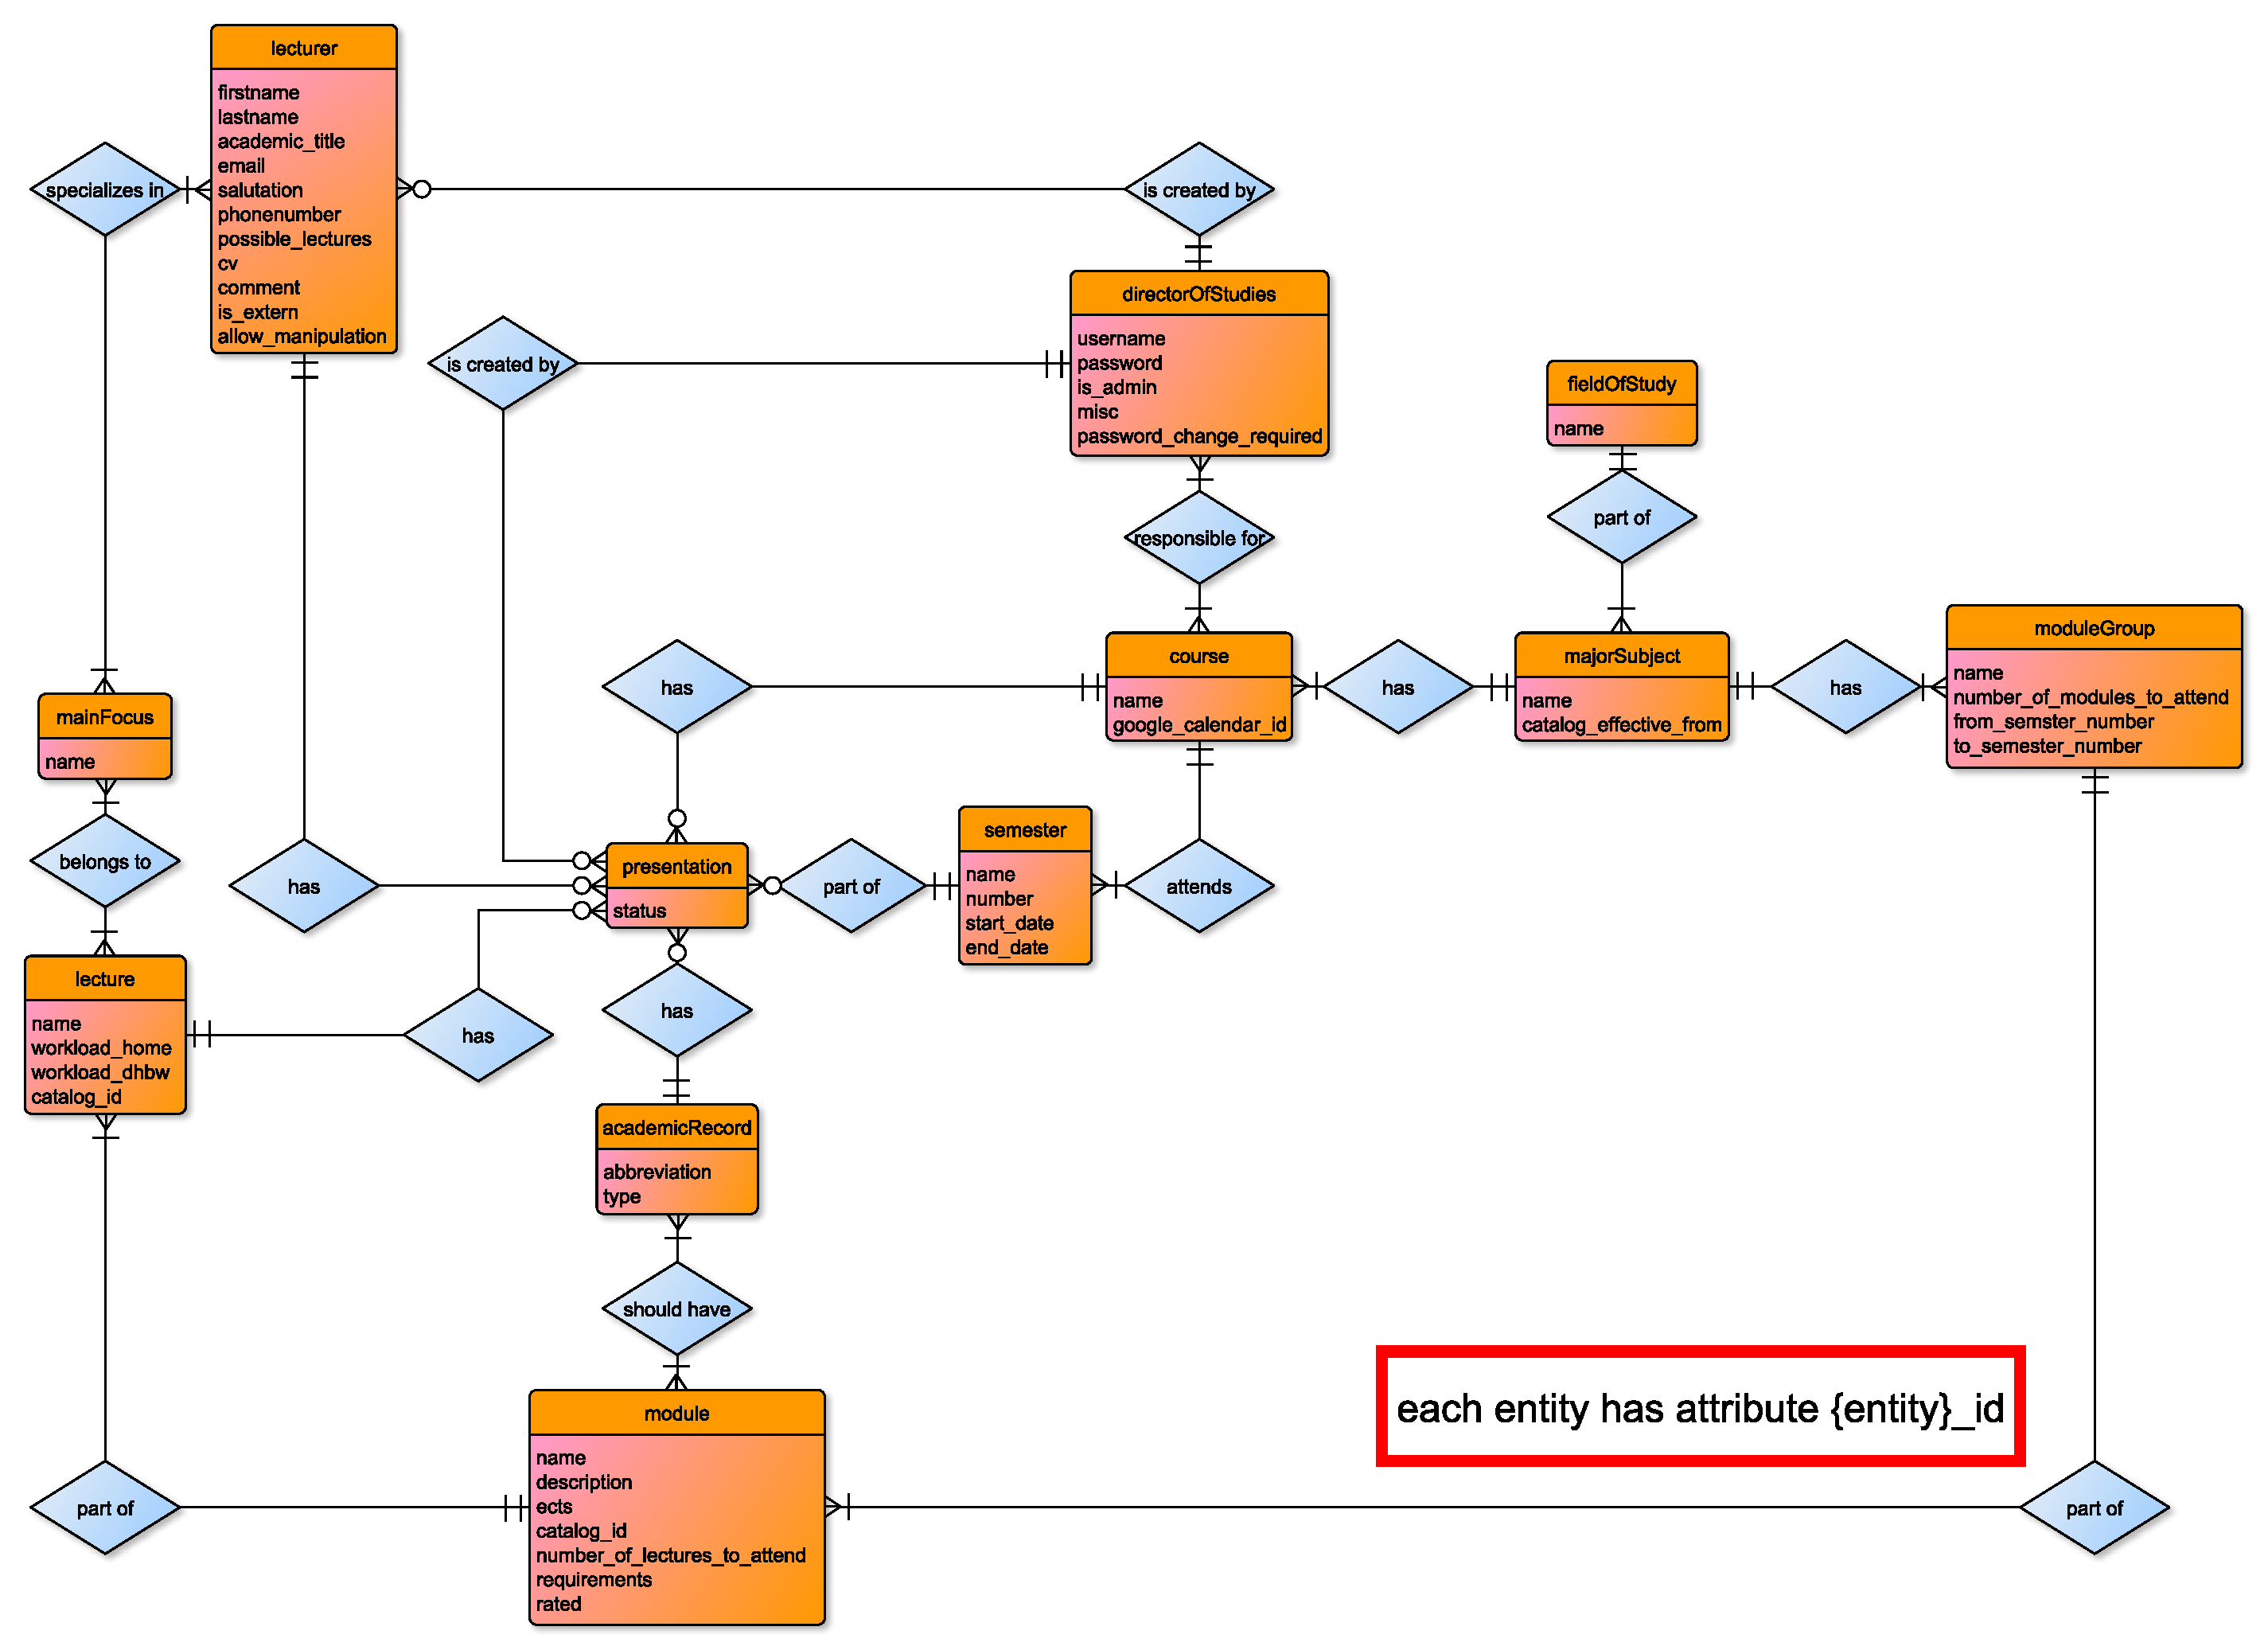
\includegraphics[angle={90}, width=0.78\textwidth]{img/er-model.pdf}
\end{figure}


\chapter{Styleguide}\label{an:Styleguide}
\begin{figure}[H]
	\centering 
	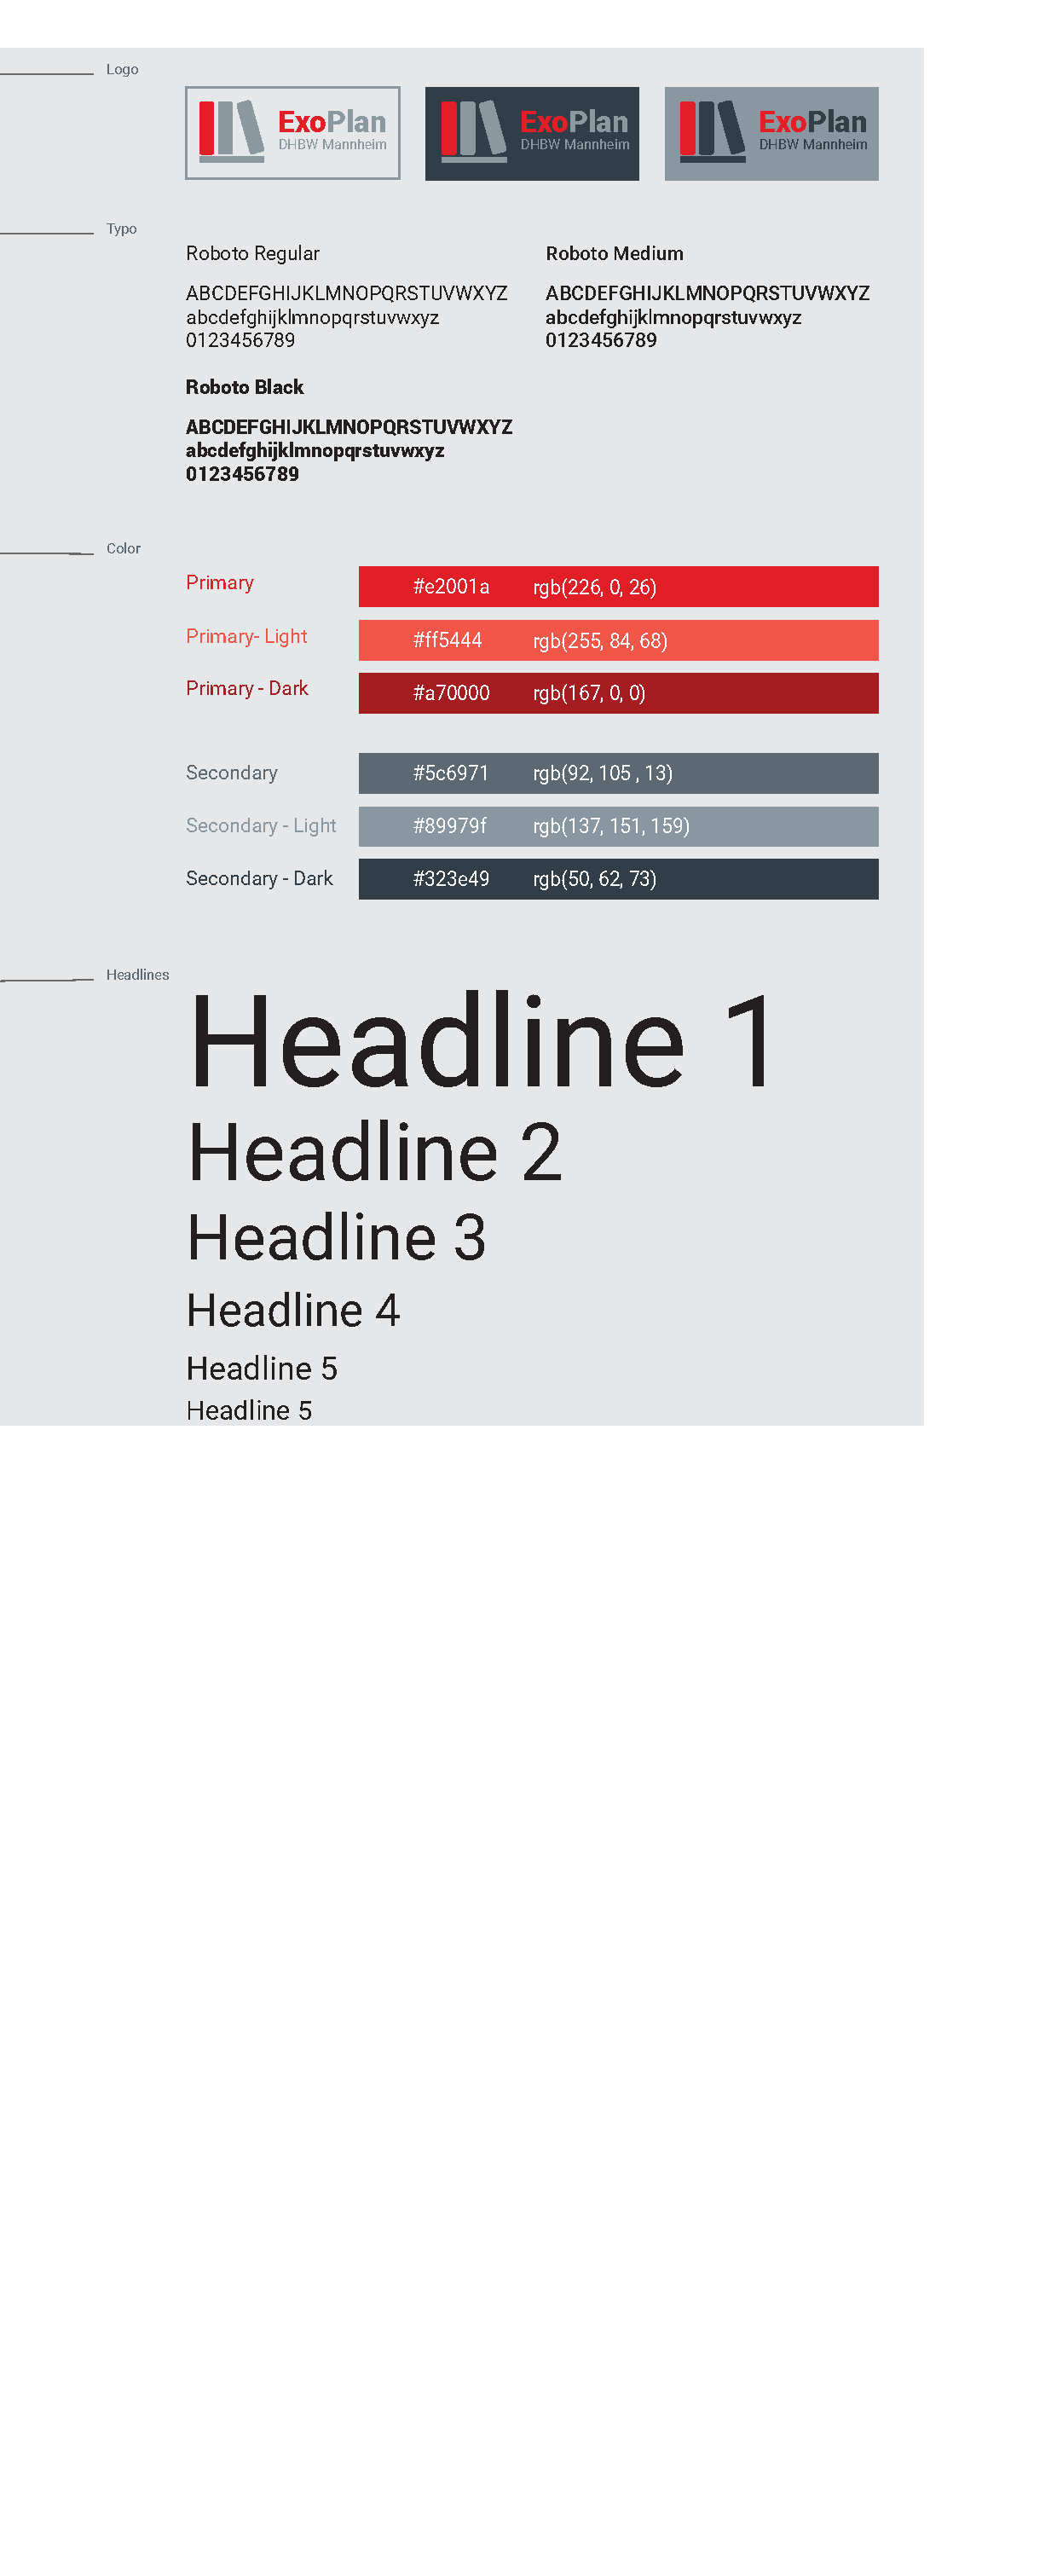
\includegraphics[page=1, width=12.5cm ]{docs/StyleguideEx.pdf}
\end{figure}

\begin{figure}[H]
	\centering 
	\includegraphics[page=2, width=12.5cm ]{docs/StyleguideEx.pdf}
\end{figure}





\end{document}